%%%\documentclass[option]{webofc}
%%% "twocolumn" for typesetting an article in two columns format (default one column)
%
\documentclass{webofc}
\usepackage[varg]{txfonts}   % Web of Conferences font
\usepackage[caption = false]{subfig}
\usepackage{float}

%
\begin{document}
%
\title{Validation of a non-thermal equilibrium Eulerian-Eulerian multiphase
model of a 620 MWe power boiler.}

\author{\firstname{Brad} \lastname{Rawlins}\inst{1}\fnsep\thanks{\email{rwlbra001@myuct.ac.za}} \and
        \firstname{Ryno} \lastname{Laubscher}\inst{2}\fnsep\thanks{\email{ryno.laubscher@uct.ac.za}} \and
        \firstname{Pieter} \lastname{Rousseau}\inst{3}\fnsep\thanks{\email{pieter.rousseau@uct.ac.za}}
        }

\institute{University of Cape Town, Department of Mechanical Engineering 
\and
           University of Cape Town, Department of Mechanical Engineering  
\and
           University of Cape Town, Department of Mechanical Engineering 
          }

\abstract{%
The use of a thermal non-equilibrium Eulerian-Eulerian model for the simulation of a 620 MWe power boiler is proposed for capturing the combustion and radiative heat transfer found in the pulverized fuel systems. The models eliminates the use of a Lagrangian reference frame in tracking solid fuel particles thereby reducing the computational expense and time. The model solves the scalar transport for the particle mass, energy and radiation interactions between the pseudo-particle and continuous phases.\\

The model is validated against both numerical and applicable site data measurements. It is shown that the model is able to adequately resolve the furnace and super-heater wall heat fluxes. Additionally the models ability to resolve the flow field, combustion dynamics and wall fluxes is demonstrated for 80\% and 60\% operational load characteristics.
}
%
\maketitle
%
\section{Introduction}
\label{intro}
The mid-merit operation of Coal-Fired Power Plants (CFPP) arises from the intermittent supply of electricity produced by renewable sources. Research into the flexible/mid-merit operation of power plants is needed to better understand the dynamic operations arising from these off-design conditions.\\
\\
Three-dimensional computational fluid dynamics (CFD) can capture the thermal performance of CFPPs at different load conditions with the necessary accuracy. These 3D CFD models include the modelling of combustion, radiation, and fluid flow phenomena. The traditional method for modelling
solid-fuel combustion systems, such as CFPPs, is acknowledged as the Eulerian-Lagrangian (EL) approach. Successful implementations, using the EL approach include the following studies \cite{bohnstein},\cite{laubscher_1} and \cite{laubscher_2}, where the later focused on the effect that the burner swirl direction has on the heat uptake to the furnace and superheater walls of a 620 MWe boiler.\\
\\
Another approach is to use a Eulerian multi-fluid model as used by the following studies \cite{epple}, \cite{cai} and \cite{wu}. Knaus et al \cite{knaus} compared the EE and EL approaches for a 550 MWe coal-fired utility boiler. The predicted combustion products yield only small differences, with carbon monoxide being better predicted when using the Eulerian-Lagrangian approach. The computational effort of the Eulerian approach proved more efficient and faster convergence times were noted.\\
\\
The current work proposes the use of an EE modelling strategy that incorporates thermal non-equilibrium between the gas and particle phases which allows for adequate particle concentration tracking and heat transfer interactions, with a reduced computational cost when compared to the EL simulation approach. The model is validated for a full scale utility power boiler for various load cases.

\section{Mathematical model} \label{Theory}
\subsection{Numerical modelling methodology}
An outline of the modelling methodology is provided in this section highlighting the general conservation equations employed, the solid phase tracking, combustion and radiation modelling techniques used in the proposed EE model. The basis of the model assumes that the gas and solid phases behave as an inter penetrating continua with both phases being described in a Eulerian reference frame. A further assumption is that the fluid is in dynamical equilibrium with the solid phase, (similar to the work of \cite{epple}), meaning that velocities of both phases are locally the same.

\subsubsection{Transport equations}
The time-averaged steady-state continuity, momentum, k-e turbulence equations and energy equations for the gas-phase can all expressed using the following generalized transport equation for a variable $\phi$ expressed as:

\begin{equation}\label{eqn_general}
\underbrace{\frac{\partial}{\partial x_{i}}(\rho u_{i}\phi)}_{\text{Convective}}= \underbrace{\frac{\partial}{\partial x_{i}}(\Gamma\frac{\partial \phi}{\partial x_{i}})}_{\text{Diffusion}}+\underbrace{S_{\phi}}_{\text{Source}} 
\end{equation}\\
The governing equations can be written as follows;\\
Mass conservation:
\begin{equation}\label{eqn_RANS_mass}
\frac{\partial}{\partial x_{i}}(\rho \bar{u}_{i})=S_{m}.
\end{equation}
Momentum conservation:
\\
\begin{equation}\label{eqn_momentum}
\frac{\partial}{\partial x_{i}}(\rho u_{i}u_{j})+\frac{\partial \overline{P}}{\partial x_{j}}=\frac{\partial}{\partial x_{i}}\left[\mu\left\{\frac{\partial u_{j}}{\partial x_{i}}+\frac{\partial u_{i}}{\partial x_{j}}-\frac{2}{3}\delta_{ij}\frac{\partial u_{i}}{\partial x_{i}}\right\}\right]+\frac{\partial}{\partial x_{i}}(-\rho\overline{u_{i}^{'}u_{j}^{'}})+S_m
\end{equation}
The momentum equation is closed off by approximating the Reynolds stresses using the Bossinesq relationship as shown in equation \ref{eqn_bouss}.
\begin{equation}\label{eqn_bouss}
-\rho\overline{u_{i}^{'}u_{j}^{'}}=\mu_{t}\left(\frac{\partial u_{i}}{\partial x_{j}}+\frac{\partial u_{j}}{\partial x_{i}}\right)-\frac{2}{3}\left(\rho k+\mu_{t}\delta_{ij}\frac{\partial u_{k}}{\partial x_{k}}\right)
\end{equation}
\\
This approximation is used in conjunction with the realizable k-e turbulence model \cite{shih} in this study, taking advantage of the low computational cost associated with the two-equation turbulence models. 
\\
\\
Energy conservation:
\begin{equation}\label{eqn_energy}
\frac{\partial }{\partial x_{i}} (u_{i}[\rho E+P])=\frac{\partial }{\partial x_{j}}\left[\lambda\frac{\partial T_{g}}{\partial x_{j}}\right] +S_{h}
\end{equation}
\\
Species transport:
\begin{equation}\label{eqn_species}
\begin{split}
&\frac{\partial}{\partial x_{i}}(\rho u_{j}Y_{k})=-\frac{\partial}{\partial x_{j}}(\vec{J_{k}})+\dot{\omega_{k}}+S_{k}\\
&k = 1,2,3...N
\end{split}
\end{equation}
where k is the number of species present in the domain.
\subsubsection{Solid phase modelling}
The pseudo particles transported into the domain are modelled using a scalar field and transported through the computational domain according equation \ref{eqn_general}. The pseudo particle scalar fields are used to define the fuel characteristics based on the proximate analysis composition (refer to table \ref{tab_fuel}), namely consisting being moisture, volatile matter, fixed  carbon and ash. Each scalar field equation are given in table \ref{tab_scalars}.\\

\begin{table}[h!]
\centering
\caption{Scalar field equation descriptions}\label{tab_scalars}       
\begin{tabular}{lll}
\hline
Variable &Description& Transport equation \\
\hline
$\phi_{mp0}$ &Original/initial mass of particles& $\frac{\partial}{\partial x_{i}}(\rho u_{i} \phi_{mp0})=0$\\
$\phi_{M}$&Moisture present in particles&$\frac{\partial}{\partial x_{i}}(\rho u_{i} \phi_{M})=\frac{1}{V} \frac{dM_{evap}}{dt}$\\
$\phi_{VM}$&Volatile matter present in particles&  $\frac{\partial}{\partial x_{i}}(\rho u_{i} \phi_{VM})=\frac{1}{V}\frac{dM_{devol}}{dt}$\\
$\phi_{FC}$&Fixed carbon present in particles&$\frac{\partial}{\partial x_{i}}(\rho u_{i} \phi_{FC})=\frac{1}{V}\frac{dM_c}{dt}$\\
$\phi_{ASH}$&Ash present in particles&$\frac{\partial}{\partial x_{i}}(\rho u_{i} \phi_{ASH})=0$\\
$\phi_{hp}$&Enthalpy of particle&Equation \ref{eqn_phi_hp}\\
\hline
\end{tabular}
\end{table}

The energy transport of the pseudo particle, is transported by defining the particle enthalpy using the following equation:
\begin{equation}\label{eqn_phi_hp}
\frac{\partial}{\partial x_{i}}(\rho u_{i} \phi_{hp})=\left(f_{heat}\frac{dM_{c}}{dt}h_{rxn} + \dot{Q}_{rad} + \dot{Q}_{conv} - \frac{dM_{evap}}{dt}h_{fg}\right)\frac{1}{V}
\end{equation}
\\
The equation accounts for all the processes associated with energy transport to the particle, giving the model the ability to track the particle temperature in the domain, moving the model away from the thermal non-equilibrium approach incorporated by previous studies using an EE approach (\cite{epple}, \cite{knaus}). The importance of the the particle temperature is important in describing the sequential steps found in modelling combustion processes.

\subsubsection{Combustion modelling}
The combustion modelling of coal is comprised of four sequential steps, namely the heating/cooling of the particles, evaporation, devolatilization and char oxidation. The process starts with the pseudo-particles entering the domain and heating up until the moistures boiling temperature of 373 K is reached \cite{cengel}. The realization of the boiling temperature would release moisture based on a boiling rate which is defined as:
\\
\begin{equation}\label{eqn_evap_release}
\frac{dM_{evap}}{dt}h_{fg}=\dot{Q}_{rad} + \dot{Q}_{conv}.
\end{equation}
\\
Following this is the devolatilization process whereby the 'volatiles' present in the fuel are liberated. The initialization temperature of the devolatilization process was found to vary between $280 - 350\;^{\circ}C$ for a variety of coals by Ranade and Gupta \cite{gupta}, thus particle heating would need to ensue after the moisture evaporation to bring the particles to the initialization temperature. A single-step Arrhenius kinetic rate model is used to approximate the devolatilization process since these models can predict the devolatilization of coal and are simpler to implement, according to Sankar et al \cite{sankar}). The rate is expressed in equation \ref{eqn_vol_release} as:\\
\begin{equation}\label{eqn_vol_release}
\frac{dM_{vol}}{dt}=R_{vol}(m_{0,vol}-m_{vol}).
\end{equation}\\
The final step of the solid fuel combustion process is realized when all the volatiles have been driven off of the pseudo-particles. The product species of the char oxidation process is CO, with 100\% of the resultant heat being absorbed by the pseudo-particle contributing to the energy rise of the particle matter in a cell. The char oxidation rate is derived from the works of Baum and Street \cite{baum} and Spalding \cite{spalding}. The model is commonly referred to as the diffusion-kinetics limited model, written as:
\begin{equation}\label{eqn_char_release}
\frac{dm_c}{dt}=-A_{p}\frac{R_{c}R_{diff}}{R_{c}+R_{diff}}P_{O_{2}}
\end{equation}
\\
The interested reader is directed to \cite{ansys} for an in-depth derivation of the above equation. According to Sankar et al \cite{sankar}, the gas phase reactions in boilers are fast with the chemical time scales being orders of magnitude faster than turbulent mixing time scales. This leads to a mixed-is burnt assumption being adequate for species and temperature distribution predictions. The gas-phase volatile and CO reactions are approximated using the two-step global reaction shown in equation \ref{eqn_volatiles}. 

\begin{equation}\label{eqn_volatiles}
\begin{split}
&\underbrace{CH_{3.51}O_{0.78}N_{0.1106}S_{0.0466}}_{Volatiles}+1.03O_2\to CO + 1.75H_2O + 0.0466SO_{2} + 0.0553N_2\\
&CO + 0.5O_2\to CO_2
\end{split}
\end{equation}

This work makes use of the two-step finite-rate/eddy-dissipation model (FR/EDM) in ANSYS Fluent® 19.3 \cite{ansys} to calculate the gaseous reaction rates. The model calculates three rates and uses the minimum of the three values for the source term calculations.\\

Chemical reaction rate:
\begin{equation}\label{eqn_rate_chemical}
R_{r}=A_{r}exp\left(\frac{-E_{a,r}}{RT_g}\right)\left[\vartheta^{'}_{k,r}-\vartheta_{k,r}\right]\prod_{L}\left[C_{l,r}\right]^{m,r}
\end{equation}\\
Rate of turbulent production eddies dissipation:
\begin{equation}\label{eqn_rate_products}
R_{k,r,P}=\vartheta_{k,r}M_{w,k}AB\rho\frac{\varepsilon}{k}min\left(\frac{\sum_{p} Y_p}{\sum_{j}\vartheta_{j,r}M_{w,j}}\right)
\end{equation}\\
Rate of reaction eddies dissipation:
\begin{equation}\label{eqn_rate_reactants}
R_{k,r,R}=\vartheta_{k,r}M_{w,k}A\rho\frac{\varepsilon}{k}min\left(\frac{Y_R}{\varepsilon_{R,r}M_{w,R}}\right)
\end{equation}

\subsubsection{Radiation modelling}

The heat transfer to the furnace, platen and final superheater walls in the case validation is mainly due to radiation. The radiation transport for the current work was resolved using the P1 radiation model which includes the effects of particle absorption ($\alpha_p$) and scattering ($\sigma_p$) as well as gas mixture absorption ($\alpha_g$). The P1 model transport variable is the incident radiation (G - $W/m^2$), and can be written for a particle laden domain as:

\begin{equation}
\frac{\partial}{\partial x_{i}}\left(\Gamma\frac{\partial G}{\partial x_{i}}\right)=\left(\alpha_g+\alpha_p)\right)G-4\left(\alpha_g \sigma_{SB} T_{g}^4-\pi E_p \right)
\end{equation}
\\
The gas mixture absorption coefficient was calculated using the weighted sum of gray gases model (WSGGM) which accounts for the tri-atomic gases $CO_2$ and $H_2O$ as proposed by Smith et al \cite{smith}. The solid phase radiative properties (namely $\alpha_p$, $\sigma_p$ and $E_p$) were determined an equivalent Eulerian description for each expressed as:\\
\begin{equation}
\alpha_p \equiv \frac{\epsilon_{p,n}A_{proj}N_p}{V}
\end{equation}
\begin{equation}
\sigma_p \equiv (1-\epsilon_{p,n})(1-f_p)\frac{A_{proj} N_p}{V}
\end{equation} 
\begin{equation}
E_p \equiv \frac{\epsilon_{p,n}A_{proj}\sigma_{SB} T_{p}^4 N_p}{\pi V}
\end{equation}
where $N_p$ is the number of particles present based off of the average diameter pseudo particle size and $A_{proj}$ is the projected area. The particles emissivity ($\epsilon_p$) and scattering factor ($f_p$) were implemented using a variable property correlation as used in the work of Laubscher and Rousseau \cite{laubscher_3}.

\newpage
\subsection{Numerical setup and model inputs} \label{Setup}
The modelling methodology, described previously, was successfully incorporated in the modelling of a 620 MWe subcritical power boiler. Figure \ref{comp_dom} illustrates the computational domain used in this validation study highlighting the various heat receiving surfaces and inlets. The burner feeds the combustion chamber with primary and secondary air through the burners inner and outer annuli respectively. At 100\% maximum continuous rating (MCR) the primary air (PA) supplies the fuel and air at a temperature of 373 K and secondary air (SA) enters at a temperature of 577 K.\\
\begin{figure}[h!]
\centering
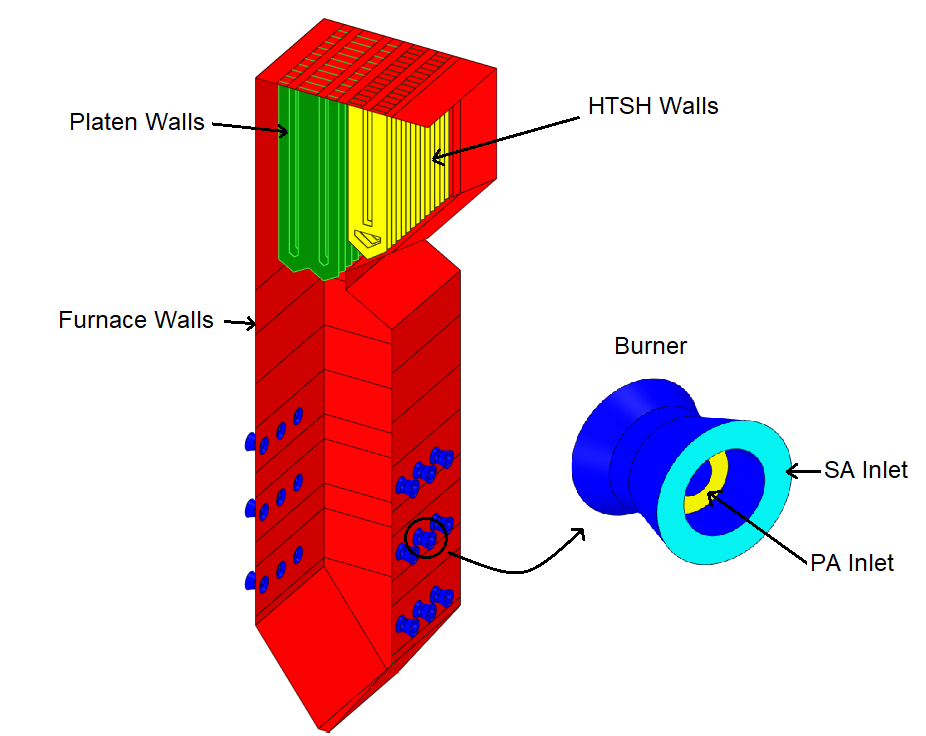
\includegraphics[scale=0.375]{domain}
\setlength{\belowcaptionskip}{0pt}
\caption{Computational domain layout}
\label{comp_dom}
\end{figure} \\
The fuel characteristics used for CFD modelling purposes are given in table \ref{tab_fuel}.
\begin{table}[h!]
\centering
\caption{Fuel characteristics used in CFD model} \label{tab_fuel}
\begin{tabular}{ll}
\hline
Fuel constituent & Fraction - ($kg/kg_{fuel}$)   \\
\hline
\textit{Ultimate analysis - [Dry-Ash-Free]} & -  \\
C & 0.775 \\
H & 0.042 \\
N & 0.018 \\
O & 0.147 \\
S & 0.018 \\
\textit{Proximate analysis - [As-received]} & -\\
Fixed Carbon & 0.34\\
Volatiles & 0.196\\
Ash & 0.409\\
H\textsubscript{2}O & 0.055\\
\hline
Energy Content & As-received - ($kJ/kg_{fuel}$)\\
\hline
HHV & 15070 \\
\hline
\end{tabular}
\end{table}\\
\\
The plant in designed to operate at a 100\% MCR with a excess air ratio of 15.5\%. As the plant is turned down from 100\% MCR the excess air ratio is increased to ensure sufficient air and fuel mixing occurs. At MCR ratings of 81\% and 60\% the excess ratios were calculated as 26.3\% and 20.9\% respectively, based off of the design schedules. The inlet flow rates and temperatures for the plants MCR rating 100\%, 81\% and 60\% are listed in table \ref{tab_inlets}.\\
\begin{table}[h!]
\centering
\caption{Inlet conditions for simulated load cases (per burner)}\label{tab_inlets}       
\begin{tabular}{llllc}
\hline
Load Rating & 100 \% & 80 \% & 60 \% & Unit  \\
\hline
PA flow rate & 4.75 & 4.01 & 2.81 & $kg/s$   \\
SA flow rate & 14.27 & 12.04 & 8.43 & $kg/s$ \\
Fuel flow rate & 3.12 & 2.52 & 1.67 & $kg/s$ \\
PA inlet temperature & 373 & 373 & 373 & $K$ \\
SA inlet temperature & 577 &558 & 535 & $K$  \\
\hline
\end{tabular}
\end{table}\\
Other necessary wall boundary conditions such as wall temperatures and emissivities are listed in the work of Laubscher and Rousseau \cite{laubscher_1}.
\subsubsection{Numerical solution strategy}
The current simulations were performed using the ANSYS Fluent\textsuperscript{\textregistered} 19.2 pressure-based solver. Pressure-momentum coupling was set to the SIMPLE technique, with momentum, energy and species equations being discretized using the second-order upwind method. The pressure equation was discretized using PRESTO!. This setup holds for both the EE model and the detailed EL model. The difference arises in the use of scalar fields in the EE configuration and using the discrete phase modelling approach in the EL setup. Simulations were performed on a numerical mesh consisting of roughly 6.2 million cells. A mesh independence study was conducted for mesh sizes consisting of 4.2 and 10.2 millions with the 6.2 million cell model deemed acceptable for this study. To ensure an accurate numerical solution the mesh aspect ratio was kept below 15 and orthogonal quality above 0.2.\\
\\
The discrete phase equations, for the EL model, were solved once every 30 fluid phase iterations. The number of particles injected per burner was set to about 7800, totalling to 140 000 particles in the entire domain.\\
\\
To ensure a stable converged solution the spatial discretization for all fields were set to first order upwind (except pressure) and solved for 1500 iterations before increasing the discretization order. The simulations were then run for a further 10000 iterations. For all cases the maximum mass imbalance was 0.046 kg/s for a tiotal gas flow rate of 376 kg/s. The maximum heat imbalance was 2450 kW for a total heat input of 855 MW.

\newpage
\section{Results and discussion} \label{Results}
The results discussed herewith compare an experimental numerical model, using the EL reference frame, to that of the developed EE modelling approach, (discussed in section \ref{Theory}) for 100\%, 81\% and 60\% MCR loads cases. Overall a 30\% decrease in simulation time was observed across the simulated load cases with a 5\% relative accuracy when using the EE model. The graphs of figure \ref{fig_heat_load} illustrate the measured plant data, numerical and EE models results,  for the heat loads to the furnace, platen and high temperature superheater (HTSH) walls. 
\begin{figure}[h!]
\centering
\subfloat[100\% load case]{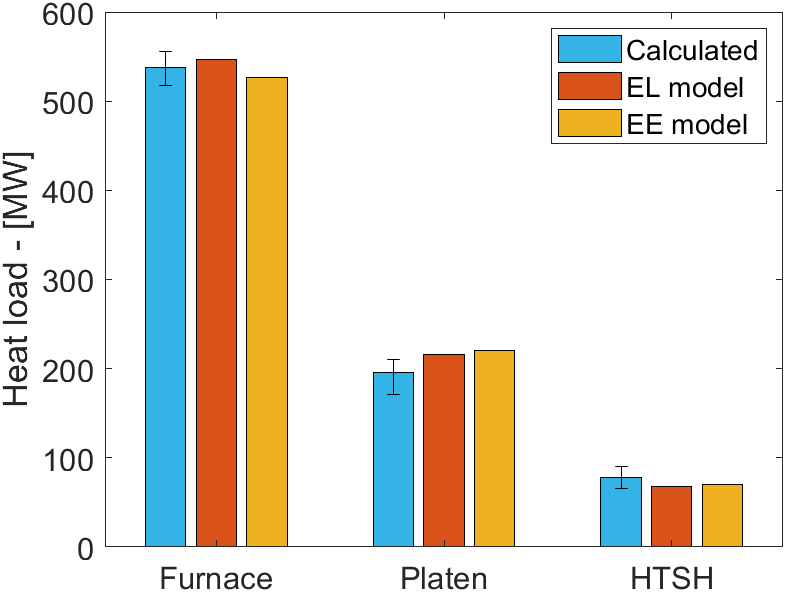
\includegraphics[width = 3.75cm, height = 3cm,  keepaspectratio]{bar_100}}
\hspace{5mm}
\subfloat[81\% load case]{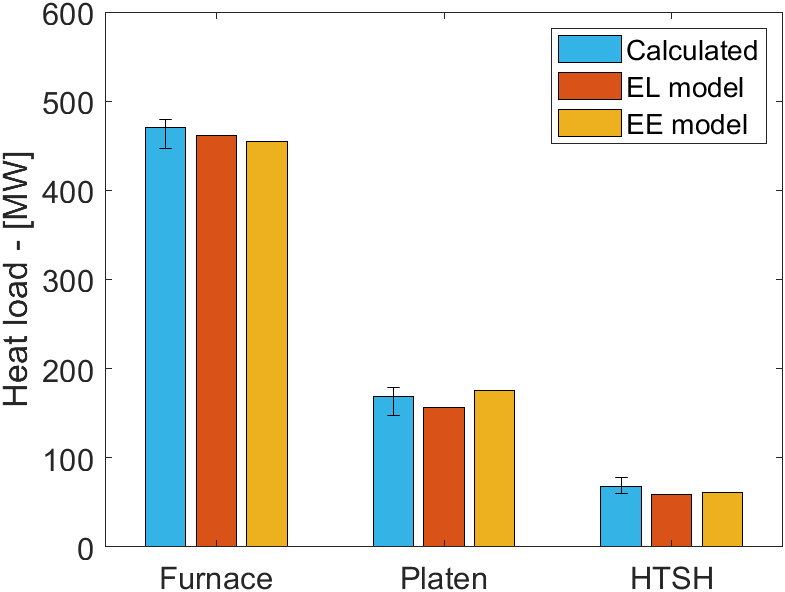
\includegraphics[width = 3.75cm, height = 3cm,  keepaspectratio]{bar_80}}
\hspace{5mm}
\subfloat[60\% load case]{\label{fig_heat_load_c}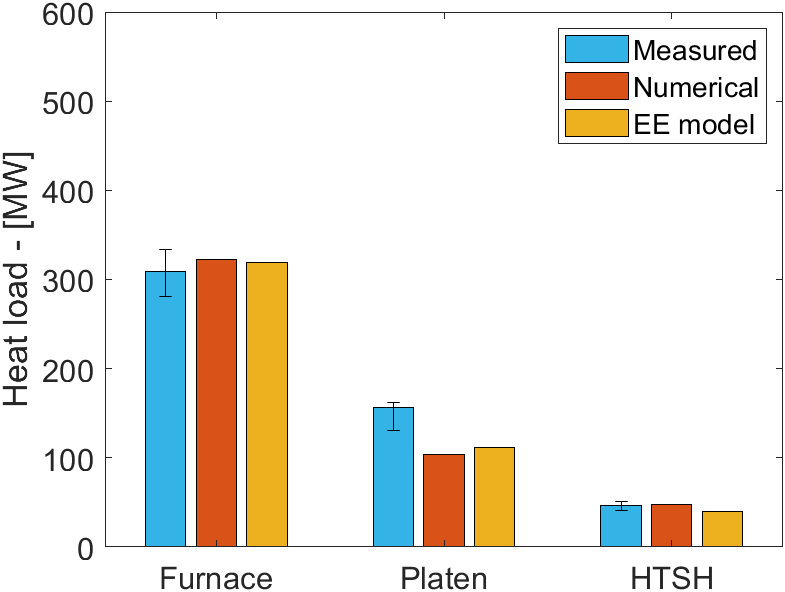
\includegraphics[width =3.75cm, height = 3cm,  keepaspectratio]{bar_60}} 
\setlength{\belowcaptionskip}{0pt}
\caption{Overall heat load performance for 100\%, 81\% and 60\% MCR load cases}
\label{fig_heat_load}
\end{figure}\\
The general accuracy of the EE model is seen to be able to sufficiently capture the overall heat loads when compared to the measured and experimental results. A notable difference is seen in the 60\% load case of figure \ref{fig_heat_load_c}, where both the experimental and EE model under-predict the platens heat load.
\begin{figure}[h!]
\centering
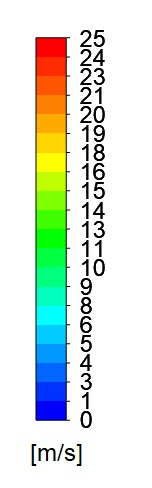
\includegraphics[scale = 0.3]{velo}
\subfloat[100\% case]{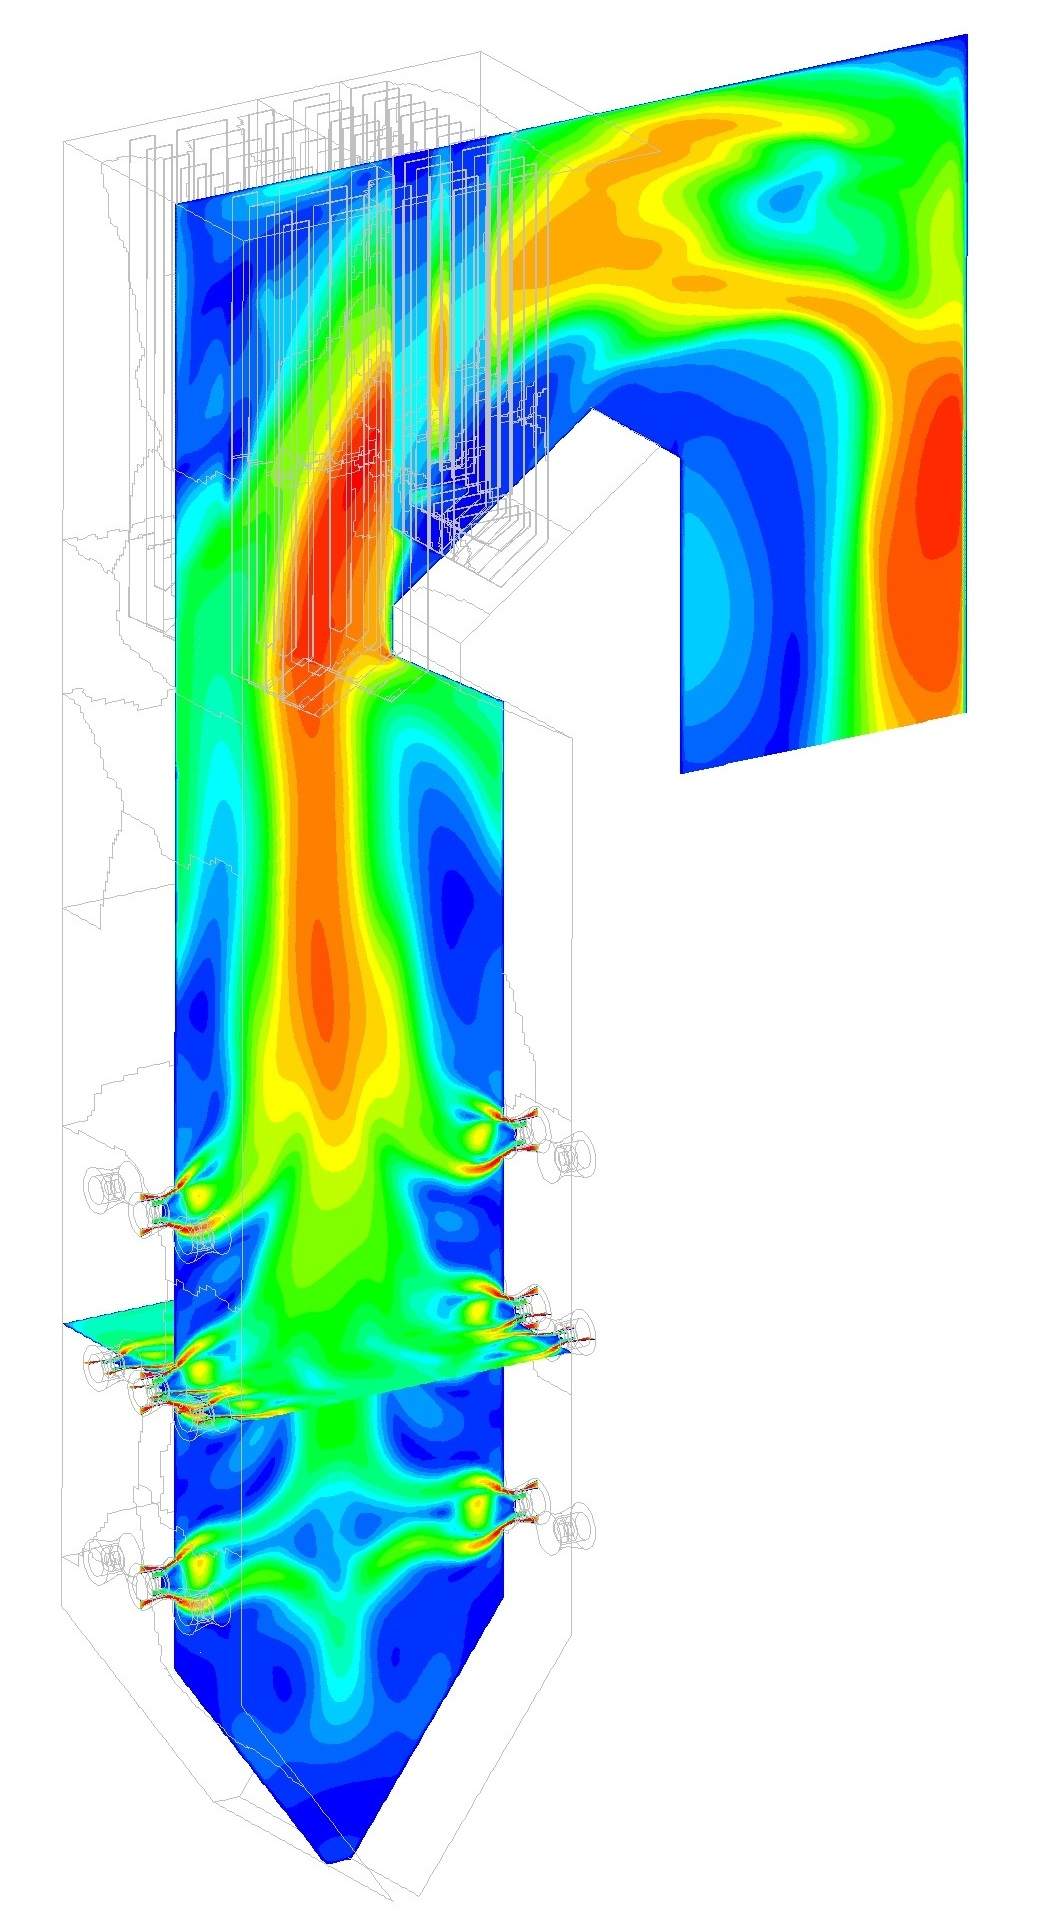
\includegraphics[scale = 0.085]{100_velo}}
\hspace{10mm} 
\subfloat[81\% case]{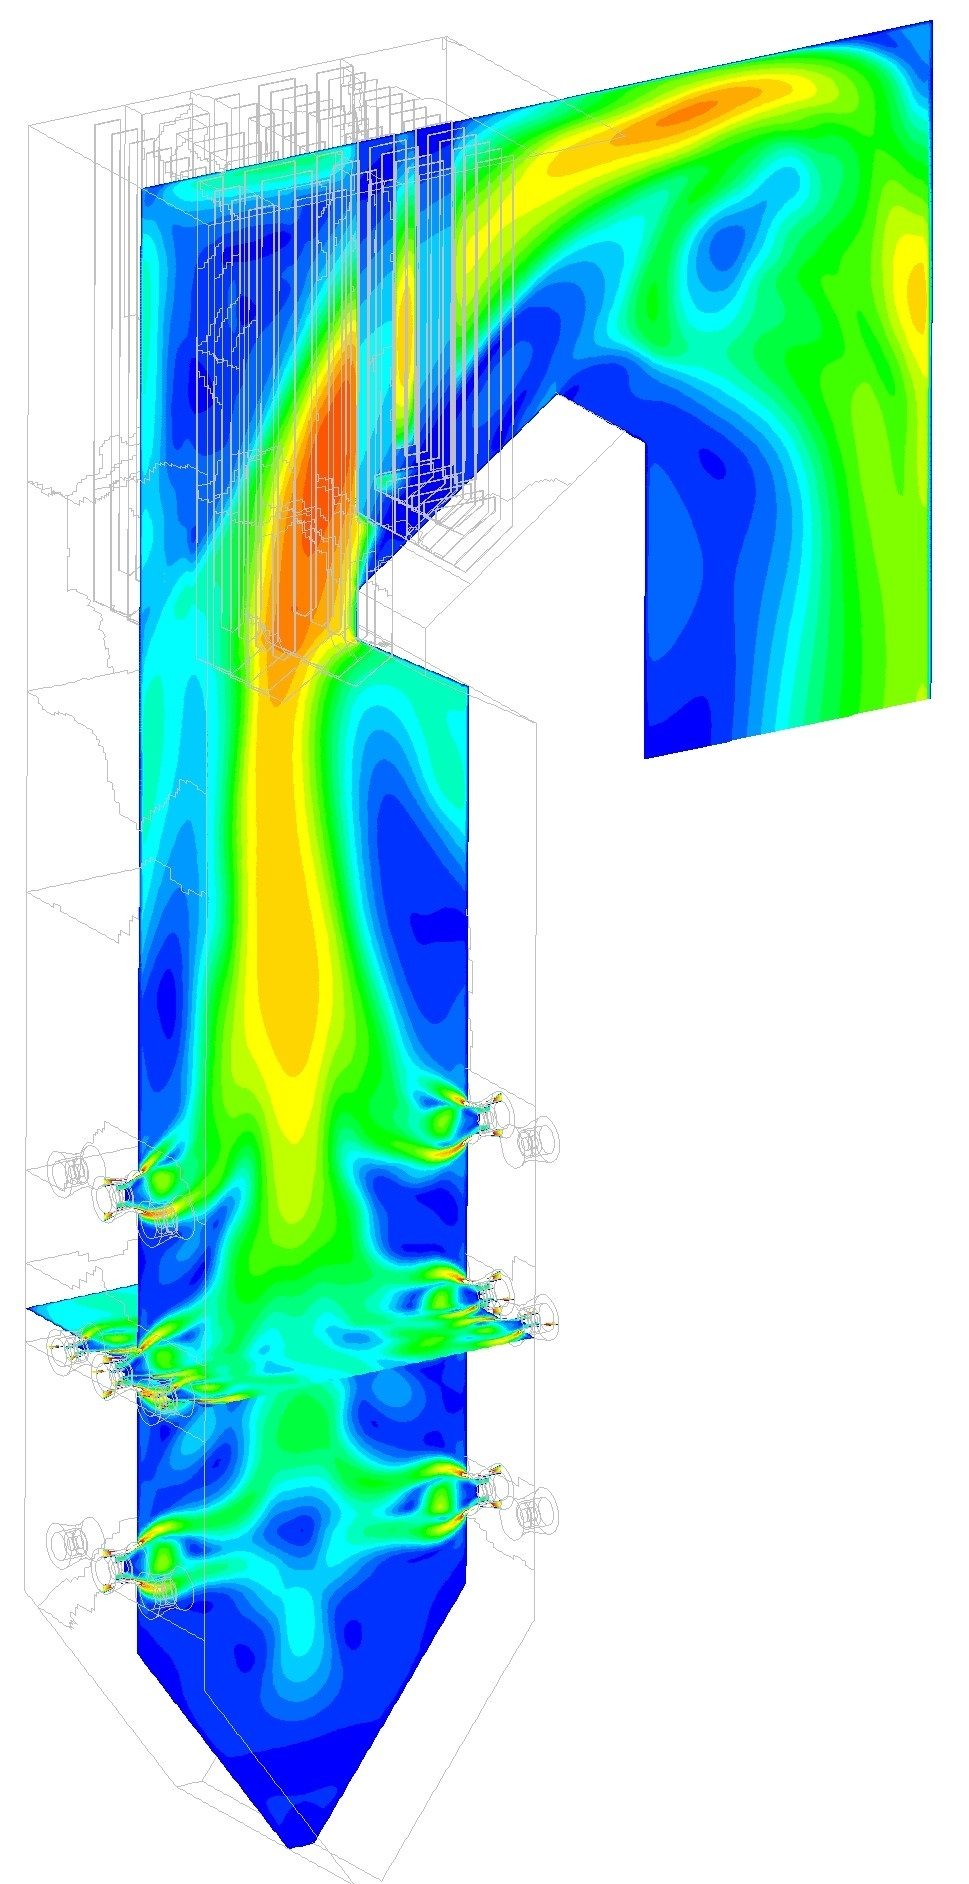
\includegraphics[scale = 0.085]{80_velo}}
\hspace{10mm} 
\subfloat[60\% case]{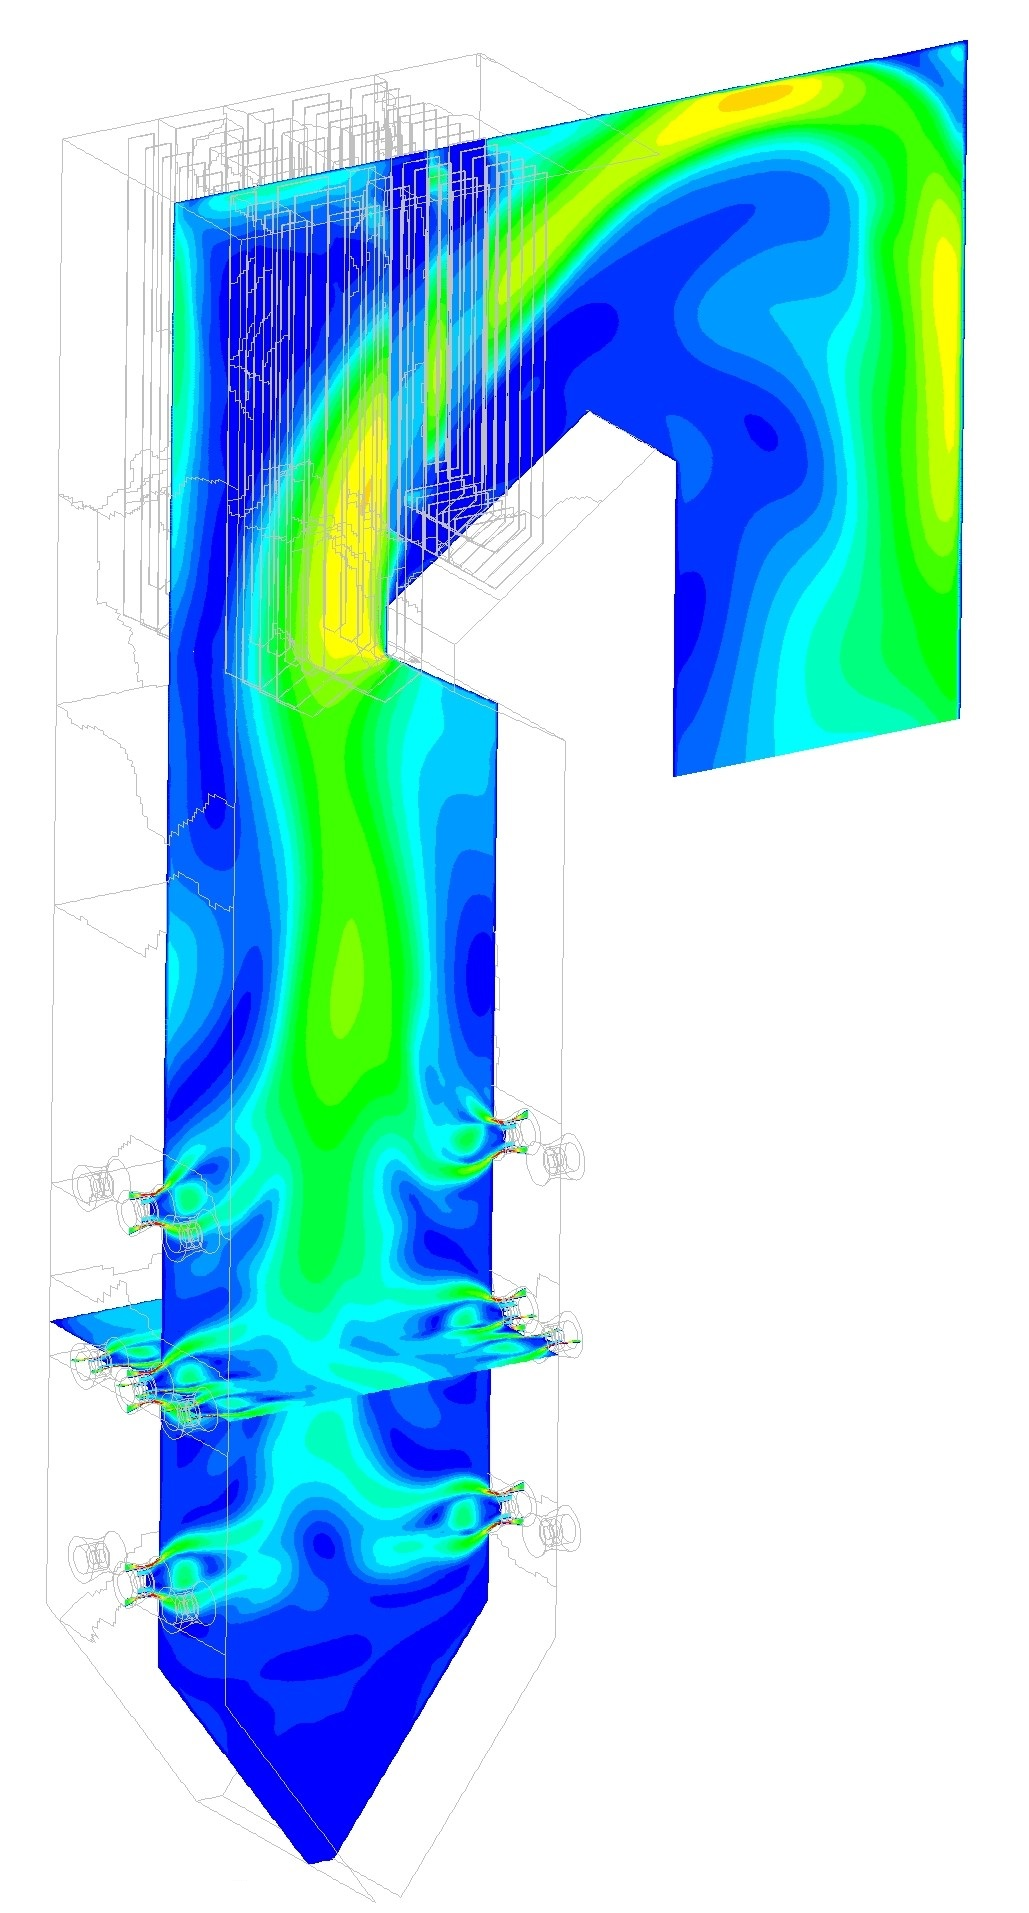
\includegraphics[scale = 0.085]{60_velo}}\\
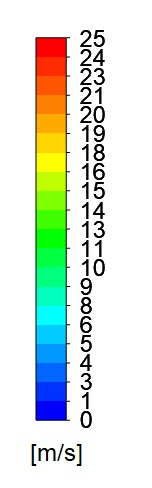
\includegraphics[scale = 0.3]{velo}
\subfloat[100\% case]{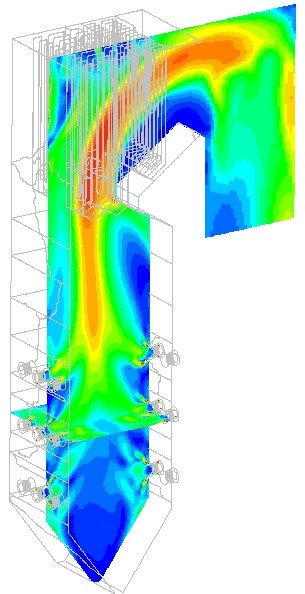
\includegraphics[scale = 0.27]{100_velo_spm}}
\hspace{10mm} 
\subfloat[81\% case]{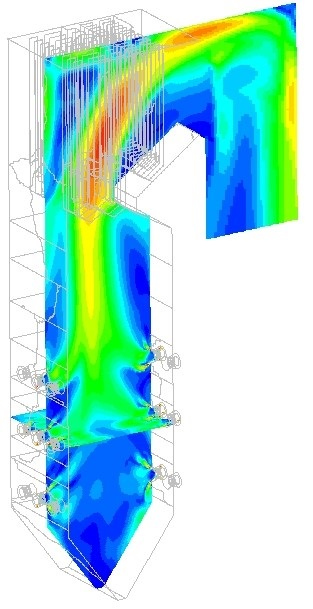
\includegraphics[scale = 0.27]{80_velo_spm}} 
\hspace{10mm} 
\subfloat[60\% case]{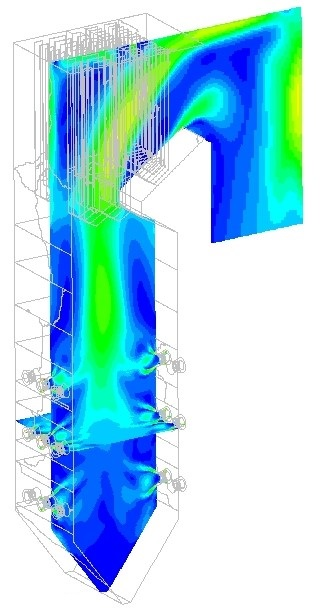
\includegraphics[scale = 0.27]{60_velo_spm}} 
\setlength{\belowcaptionskip}{0pt}
\caption{Gas velocity contour plots for the numerical (a-c) and EE model (d-f) simulated load cases}
\label{fig_velocity}
\end{figure}\\
\\
Figure \ref{fig_velocity} compares the gas velocity contour plots for the numerical and EE model. It can be seen that results are in good agreement. The EE model tends to under predict the lower burner velocity transport resulting in combustion occurring closer to the burner mouth and lower furnace walls. This effect is seen in both the temperature contour plots of figure \ref{fig_temp} (d-f) and wall heat flux contours of figure \ref{fig_wall_heat} (d-f).
\begin{figure}[h!]
\centering
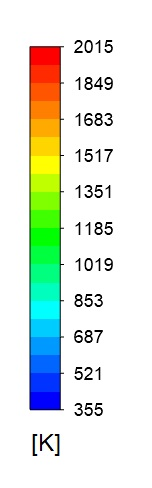
\includegraphics[scale = 0.3]{temp} 
\subfloat[100\% case]{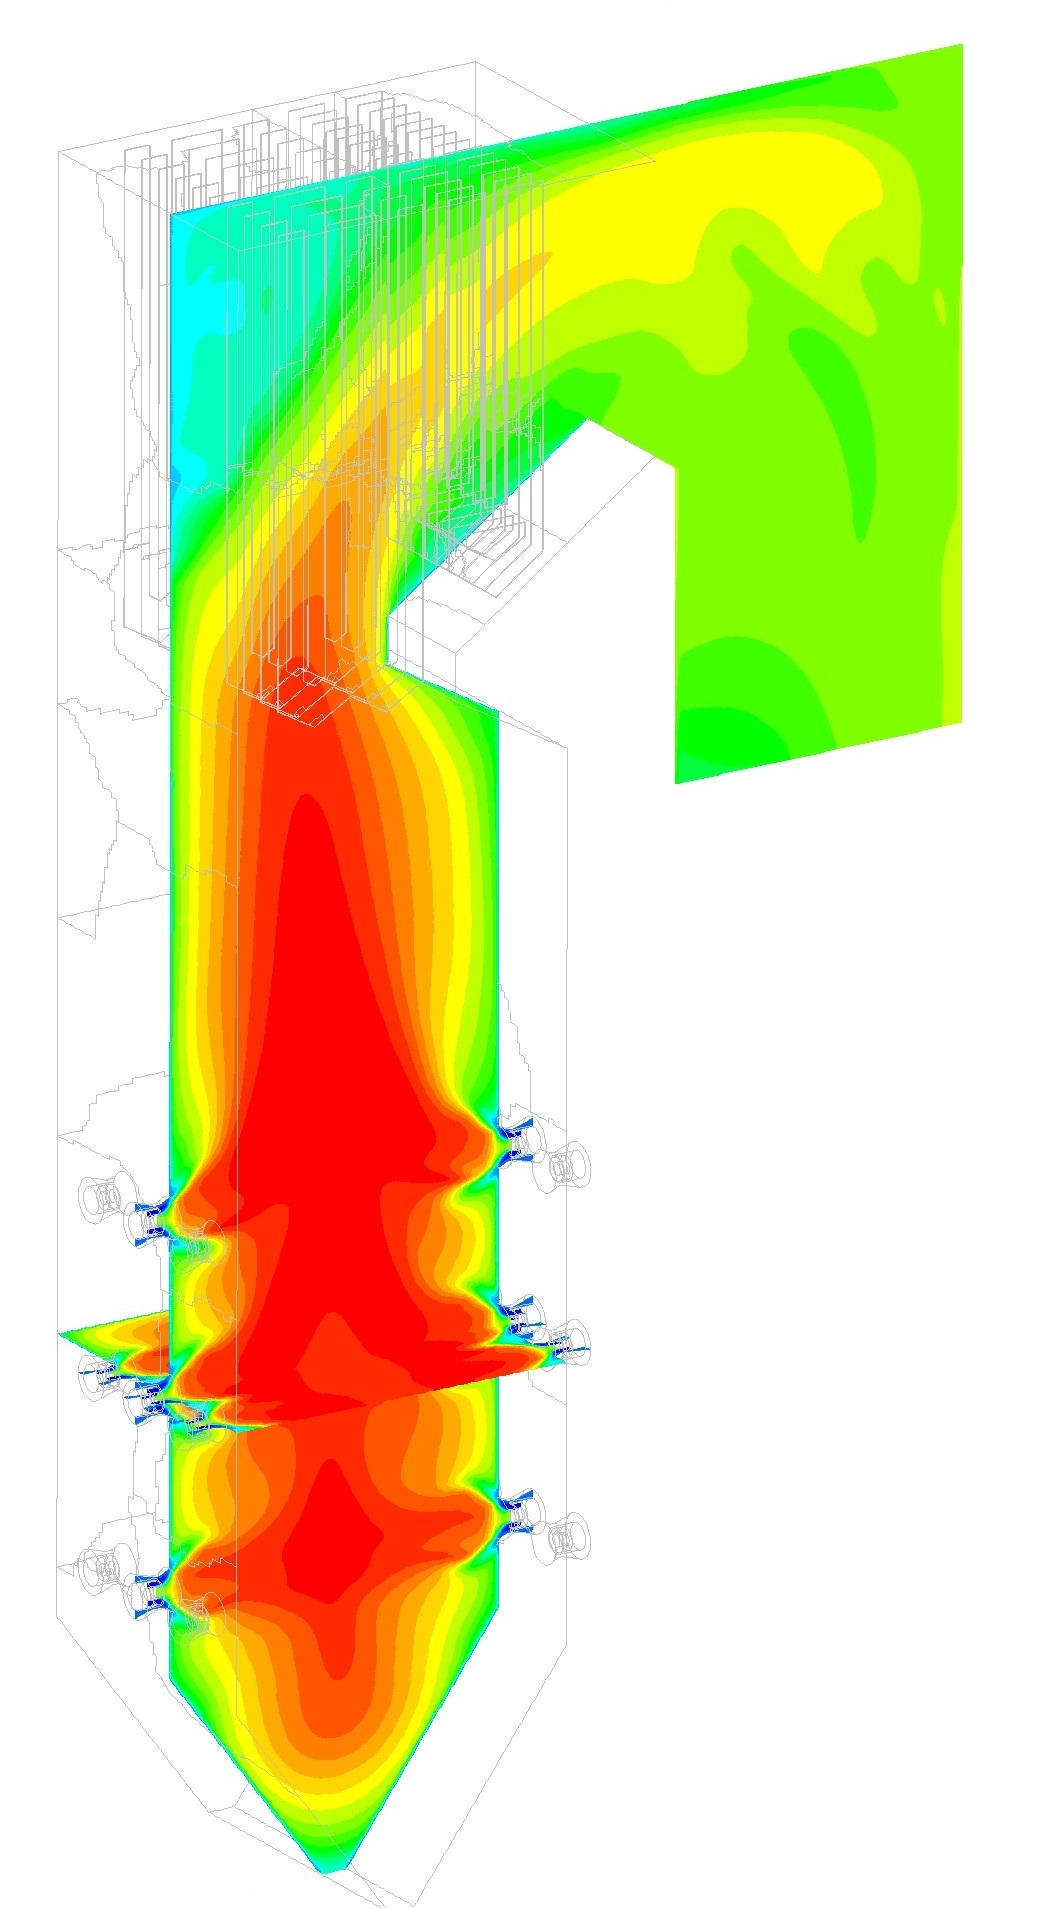
\includegraphics[scale = 0.082]{100_temp}}
\hspace{10mm}  
\subfloat[81\% case]{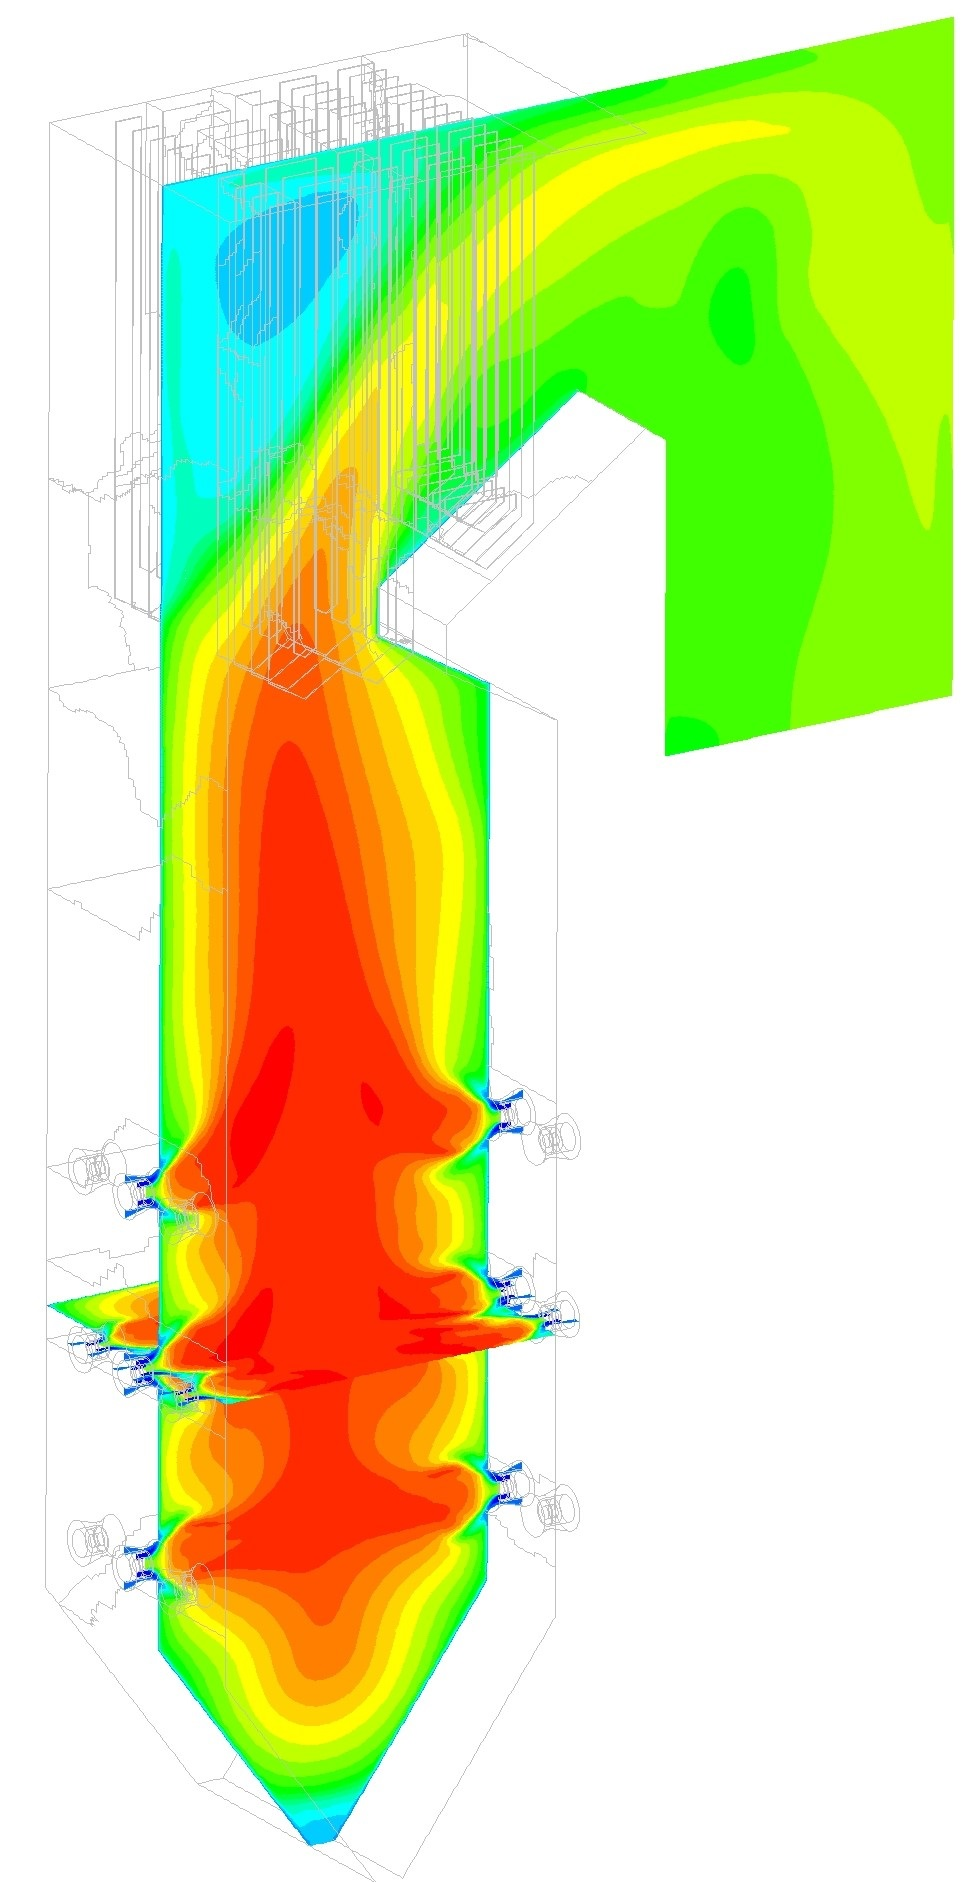
\includegraphics[scale = 0.082]{80_temp}}
\hspace{10mm} 
\subfloat[60\% case]{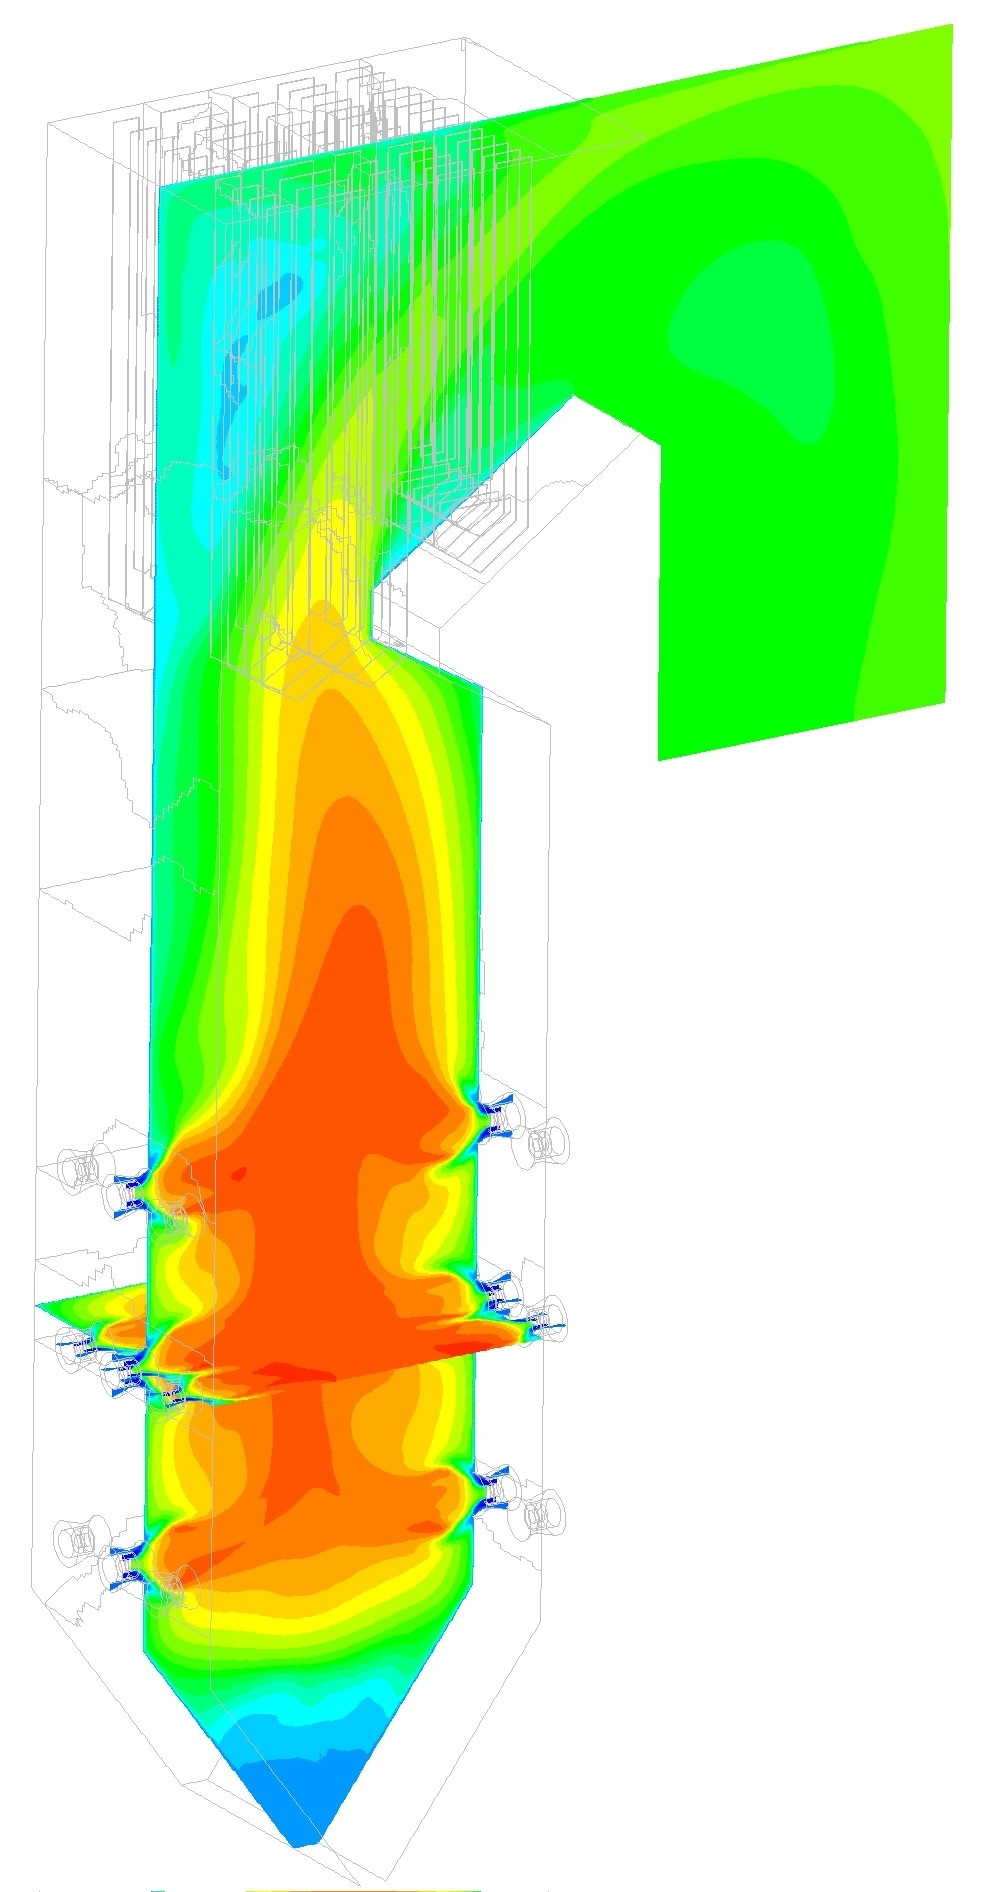
\includegraphics[scale = 0.082]{60_temp}}\\
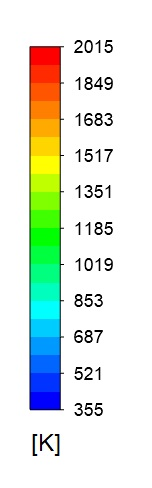
\includegraphics[scale = 0.3]{temp}
\subfloat[100\% case]{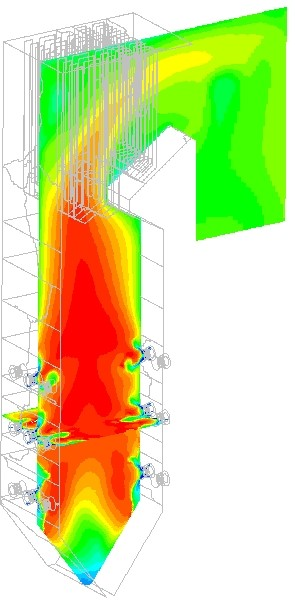
\includegraphics[scale = 0.26]{100_temp_spm}}
\hspace{10mm} 
\subfloat[81\% case]{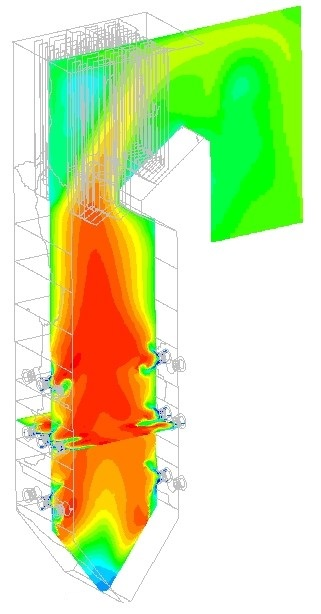
\includegraphics[scale = 0.26]{80_temp_spm}} 
\hspace{10mm} 
\subfloat[60\% case]{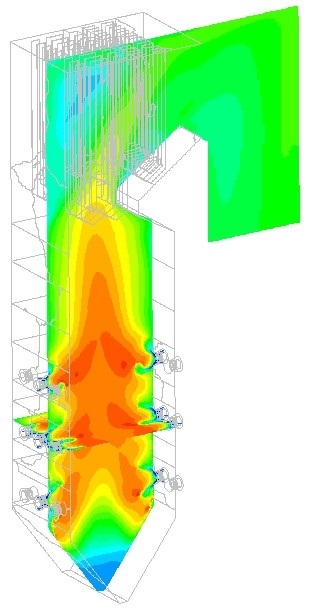
\includegraphics[scale = 0.26]{60_temp_spm}} 
\setlength{\belowcaptionskip}{0pt}
\caption{Temperature plots for the numerical (a-c) and EE model (d-f) simulated load cases}
\label{fig_temp}
\end{figure}\\
The temperature contour plots of figure \ref{fig_temp} (d-f) illustrates the EE models ability to sufficiently resolve the temperature profiles when compared to the numerical model. The lower burners tend to initiate combustion closer to the burner leading to high temperatures, due to the lack of velocity of the gas phase in this area the high temperatures  are closer to the walls of the furnace leading to a higher heat flux observed as seen in figure \ref{fig_wall_heat} (d-f). In general the temperature and velocity of profiles are deemed sufficiently accurate for the purposes of surrogate model development, since the parameter of interest is the resolution of the wall flux field.\\
\\
The heat flux profiles are given in figure \ref{fig_wall_heat} (a-f). The EE model over predicts the wall flux profiles in the lower half of the boiler, namely due to the high temperatures experienced in these zones in and around the bottom burners. The platen and HTSH radiant superheaters show a similar flux profiles with the top half of the furnace illustrating sufficient accuracy between the numerical and EE model.\\
\\
\\
\\
\\
\begin{figure}[h!]
\centering
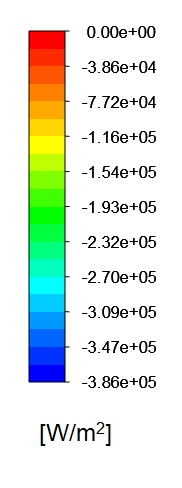
\includegraphics[scale = 0.4]{wall_heat}
\subfloat[100\% case]{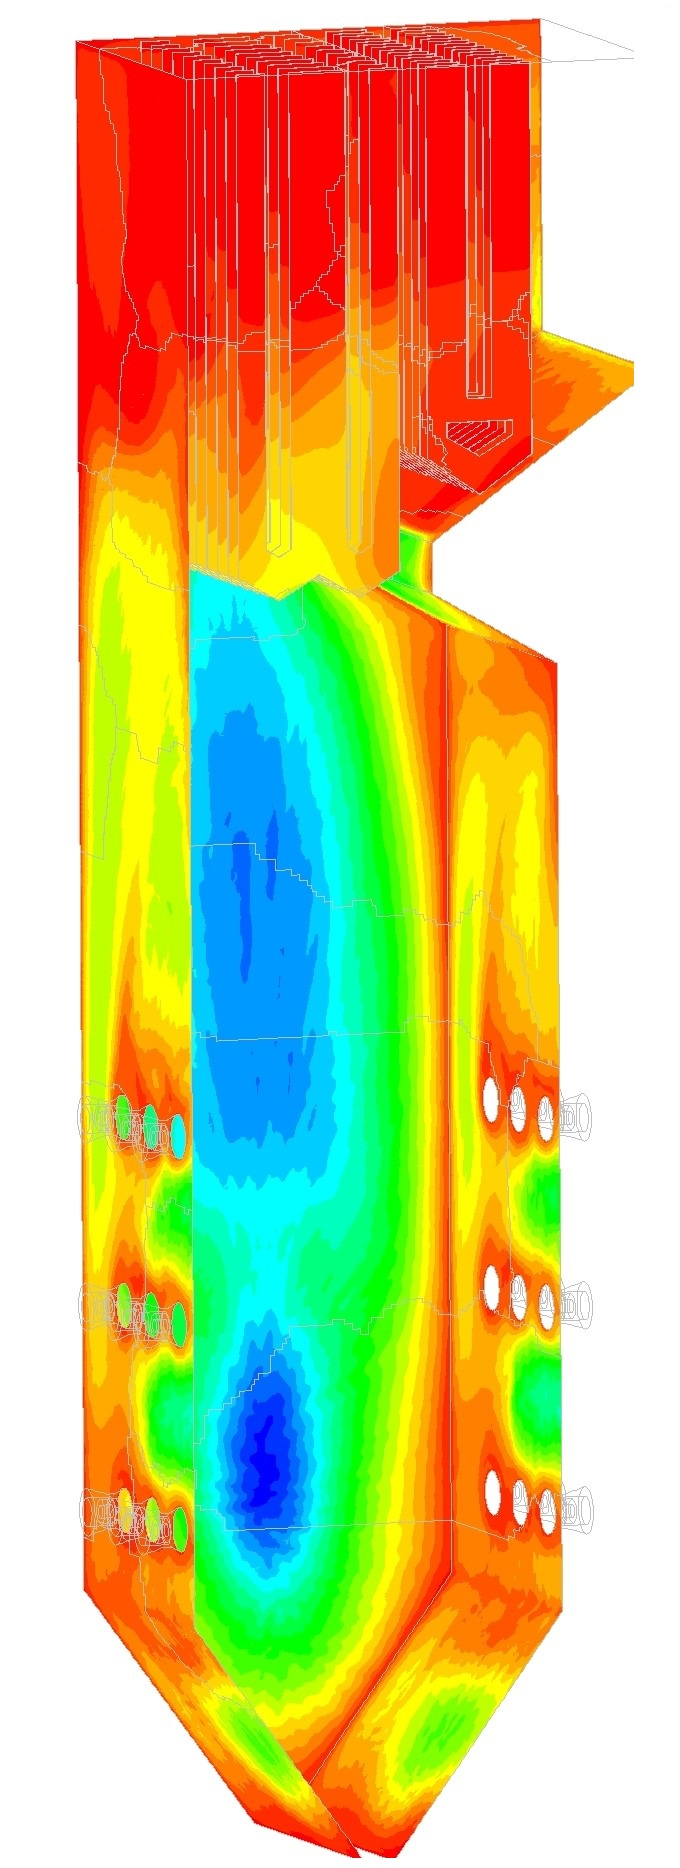
\includegraphics[scale = 0.095]{100_heat}} 
\hspace{10mm} 
\subfloat[81\% case]{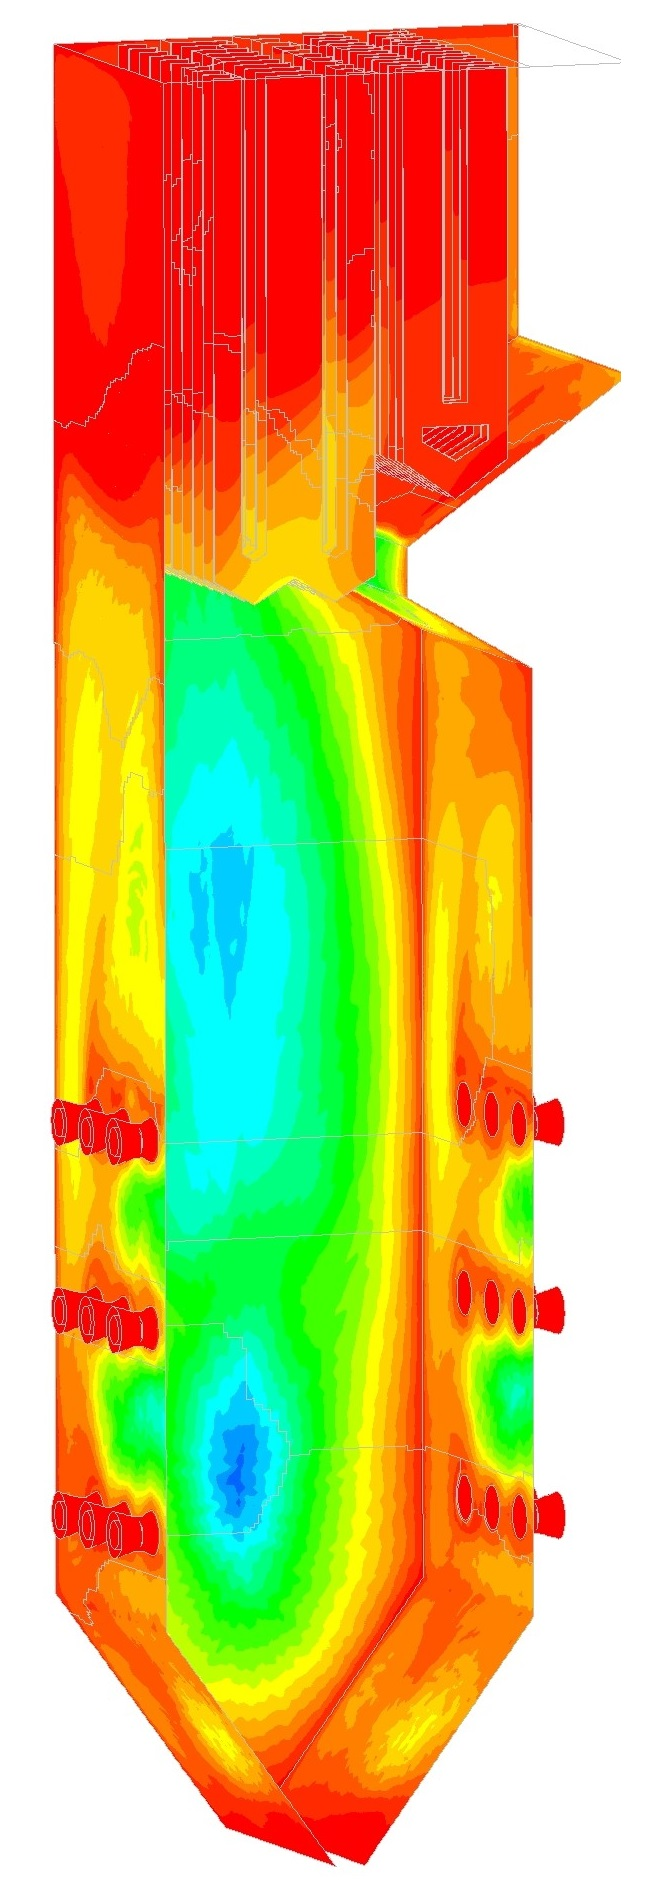
\includegraphics[scale = 0.095]{80_heat}}
\hspace{10mm} 
\subfloat[60\% case]{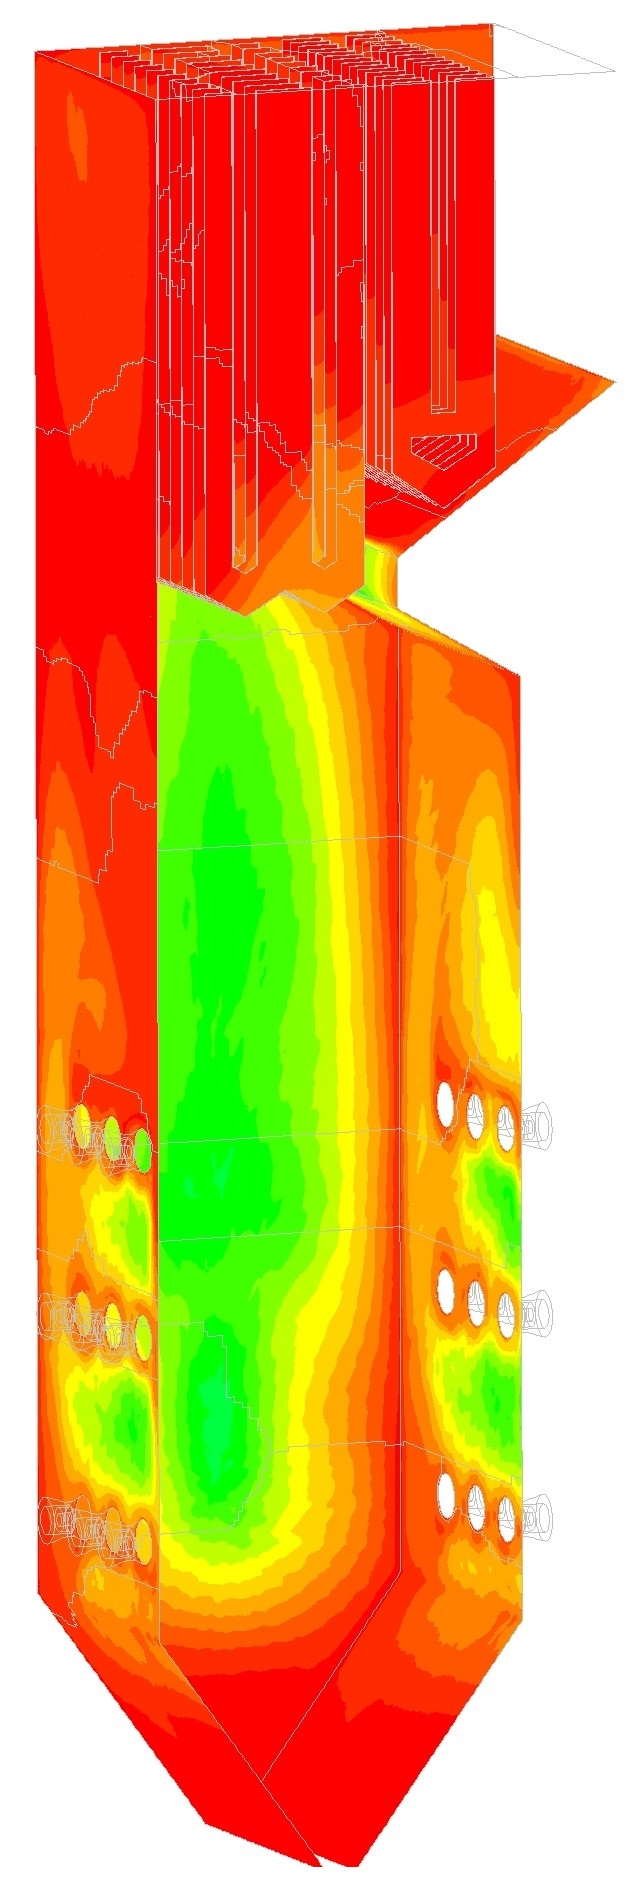
\includegraphics[scale = 0.095]{60_heat}}\\
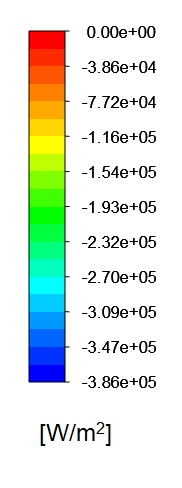
\includegraphics[scale = 0.4]{wall_heat}
\subfloat[100\% case]{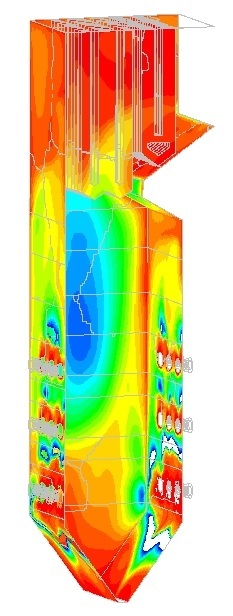
\includegraphics[scale = 0.29]{100_heat_spm}}
\hspace{10mm} 
\subfloat[81\% case]{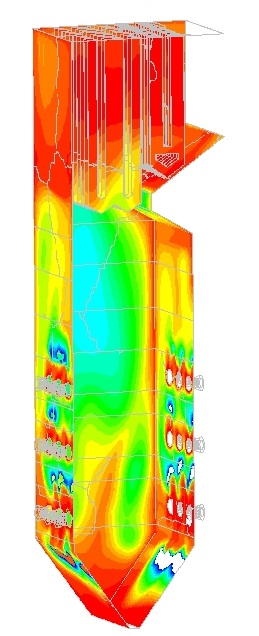
\includegraphics[scale = 0.3]{80_heat_spm}} 
\hspace{10mm} 
\subfloat[60\% case]{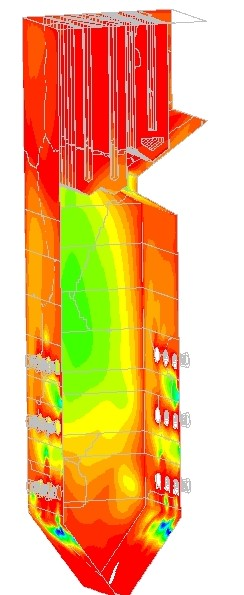
\includegraphics[scale = 0.3]{60_heat_spm}}
\setlength{\belowcaptionskip}{0pt} 
\caption{Wall heat flux profiles for the numerical (a-c) and EE model (d-f) simulated load cases}
\label{fig_wall_heat}
\end{figure}\\
Table \ref{tab_rel_err} highlights the relative errors obtained between the numerical and EE model. The maximum error of 8.15\% occurs in the platen superheater for the 100\% load case. The relative errors are deemed acceptable for the decrease in computational time required by the EE model.
\begin{table}[h!]
\centering
\caption{Relative percentage errors of key parameters between the numerical and EE models}\label{tab_rel_err}       
\begin{tabular}{llll}
\hline
Load Rating & 100\% & 80\% & 60\%   \\
\hline
Furnace heat load & 4.05\% & 8.15\% & 1.23\%   \\
Platen heat load & 6.93\% & 7.36\% & 7.21\%   \\
HTSH heat load & 2.81\% & 3.78\% & 4.23\%  \\
Furnace exit temperature & 3.56\% & 4.76\% & 5.62\%  \\
Exit X\textsubscript{CO\textsubscript{2}} fraction & 2.12\% & 1.56\% & 0.98\% \\
Exit X\textsubscript{O\textsubscript{2}} fraction & 1.86\% &3.21\% & 2.84\%\\
\hline
\end{tabular}
\end{table}\\
The spatial distribution of the particles (expressed in $kg/m^3$) of figure \ref{fig_concentration} (a-f) highlights the EE models ability to resolve the particle concentration throughout the domain for the various load cases. The general trend of the EE model is with sufficient accuracy when compared to the numerical model.\\
\begin{figure}[h!]
\centering
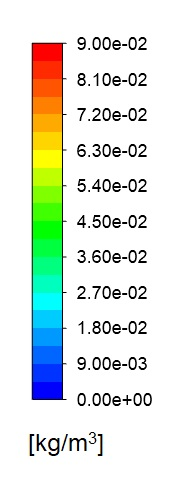
\includegraphics[scale = 0.3]{concentration}
\subfloat[100\% case]{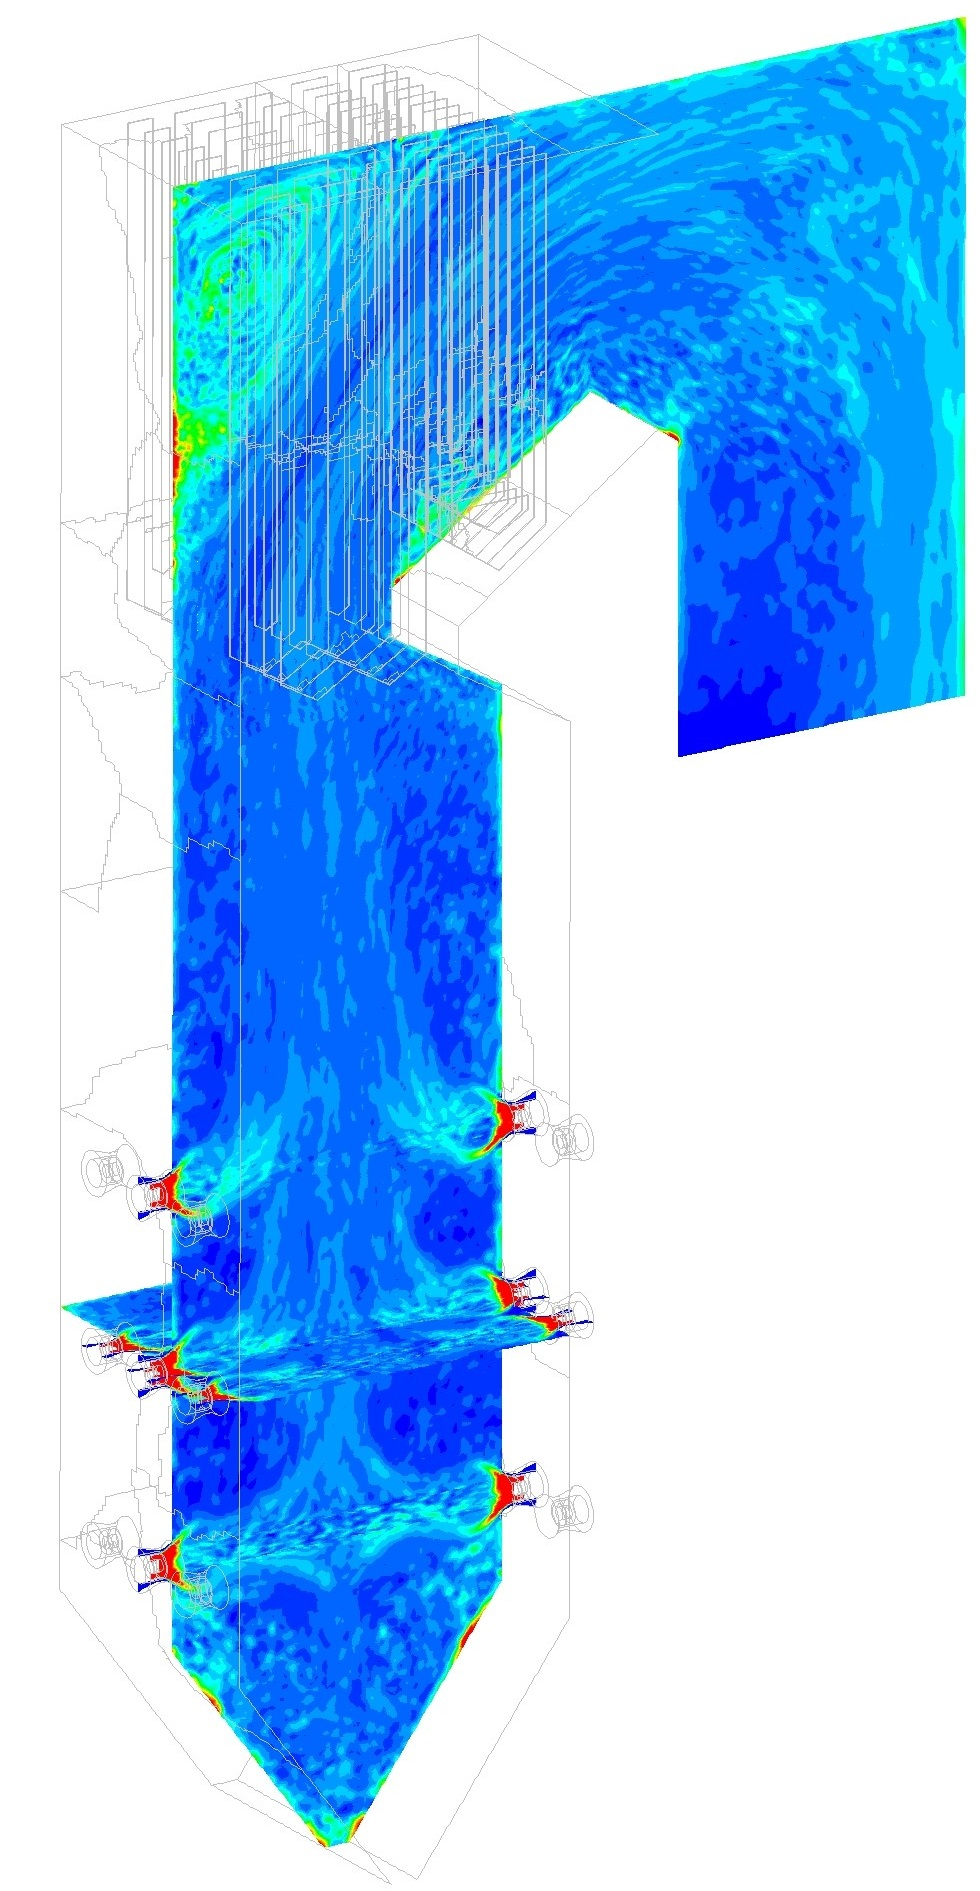
\includegraphics[scale = 0.085]{100_concentration}}
\hspace{10mm}  
\subfloat[100\% case]{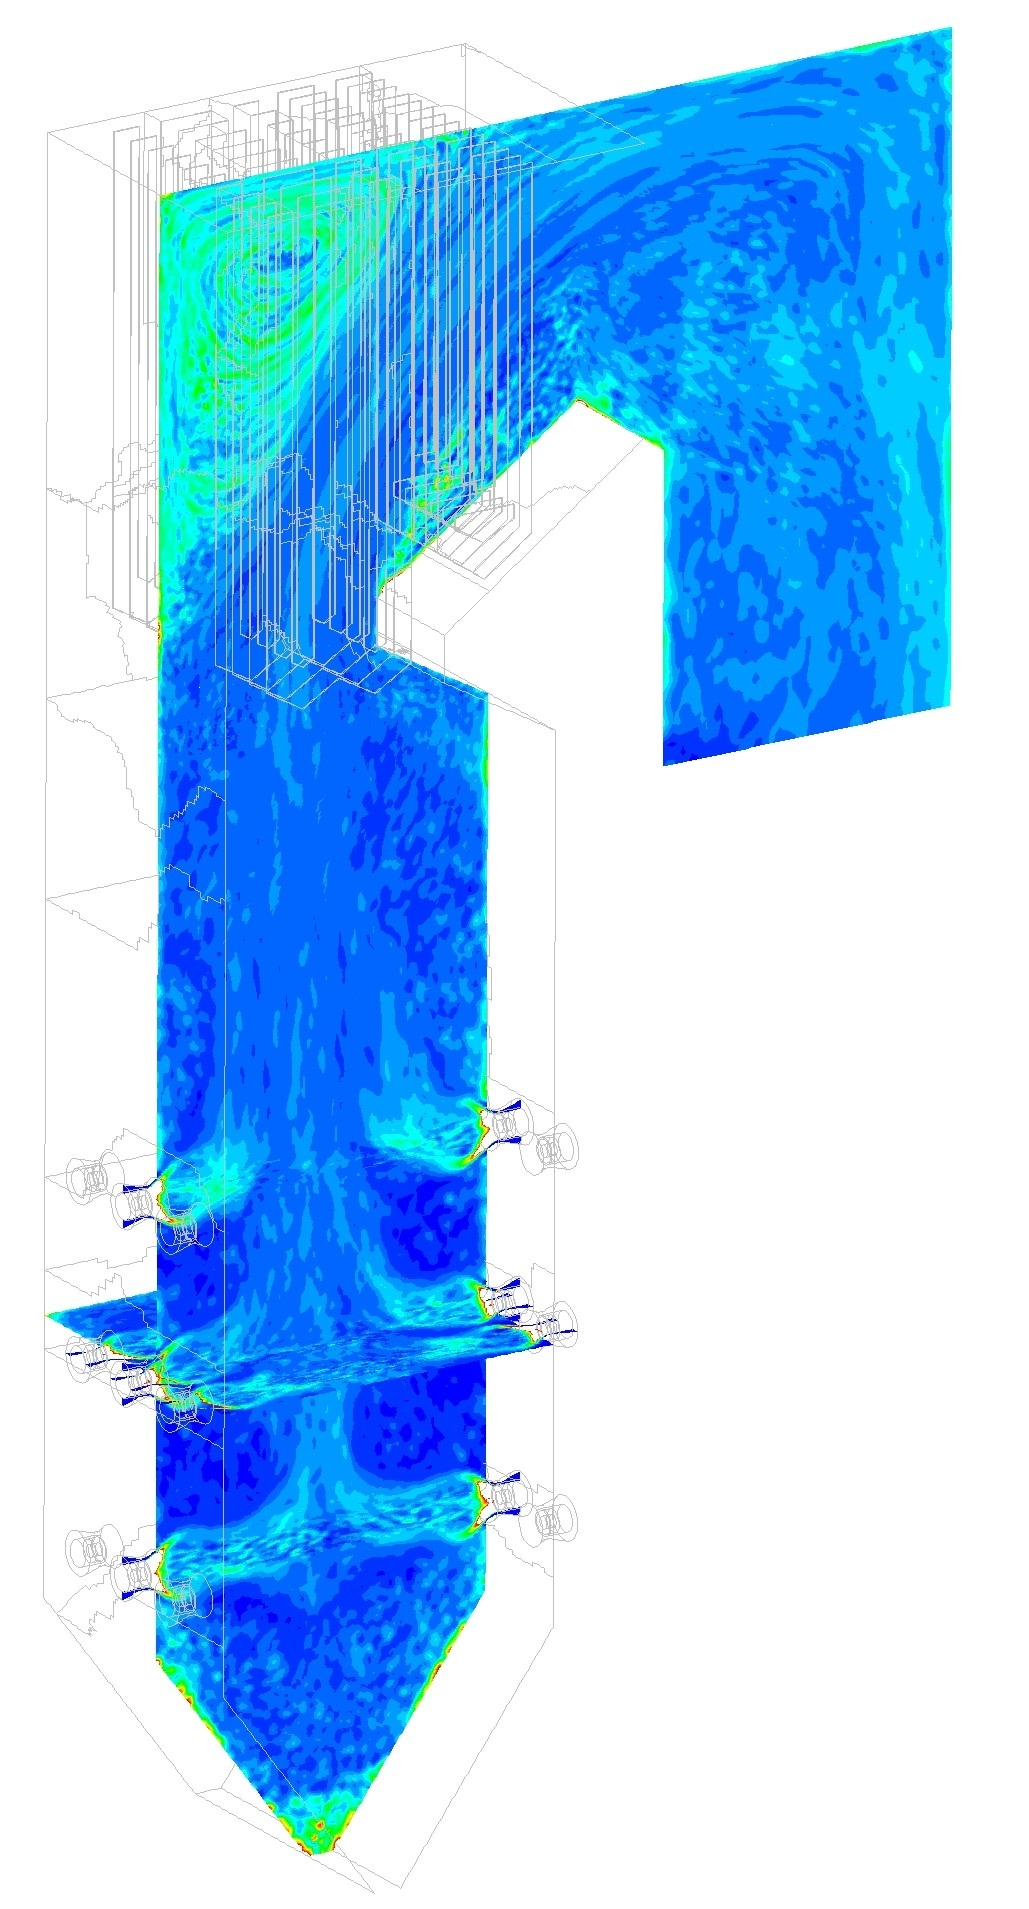
\includegraphics[scale = 0.085]{80_concentration}}
\hspace{10mm} 
\subfloat[100\% case]{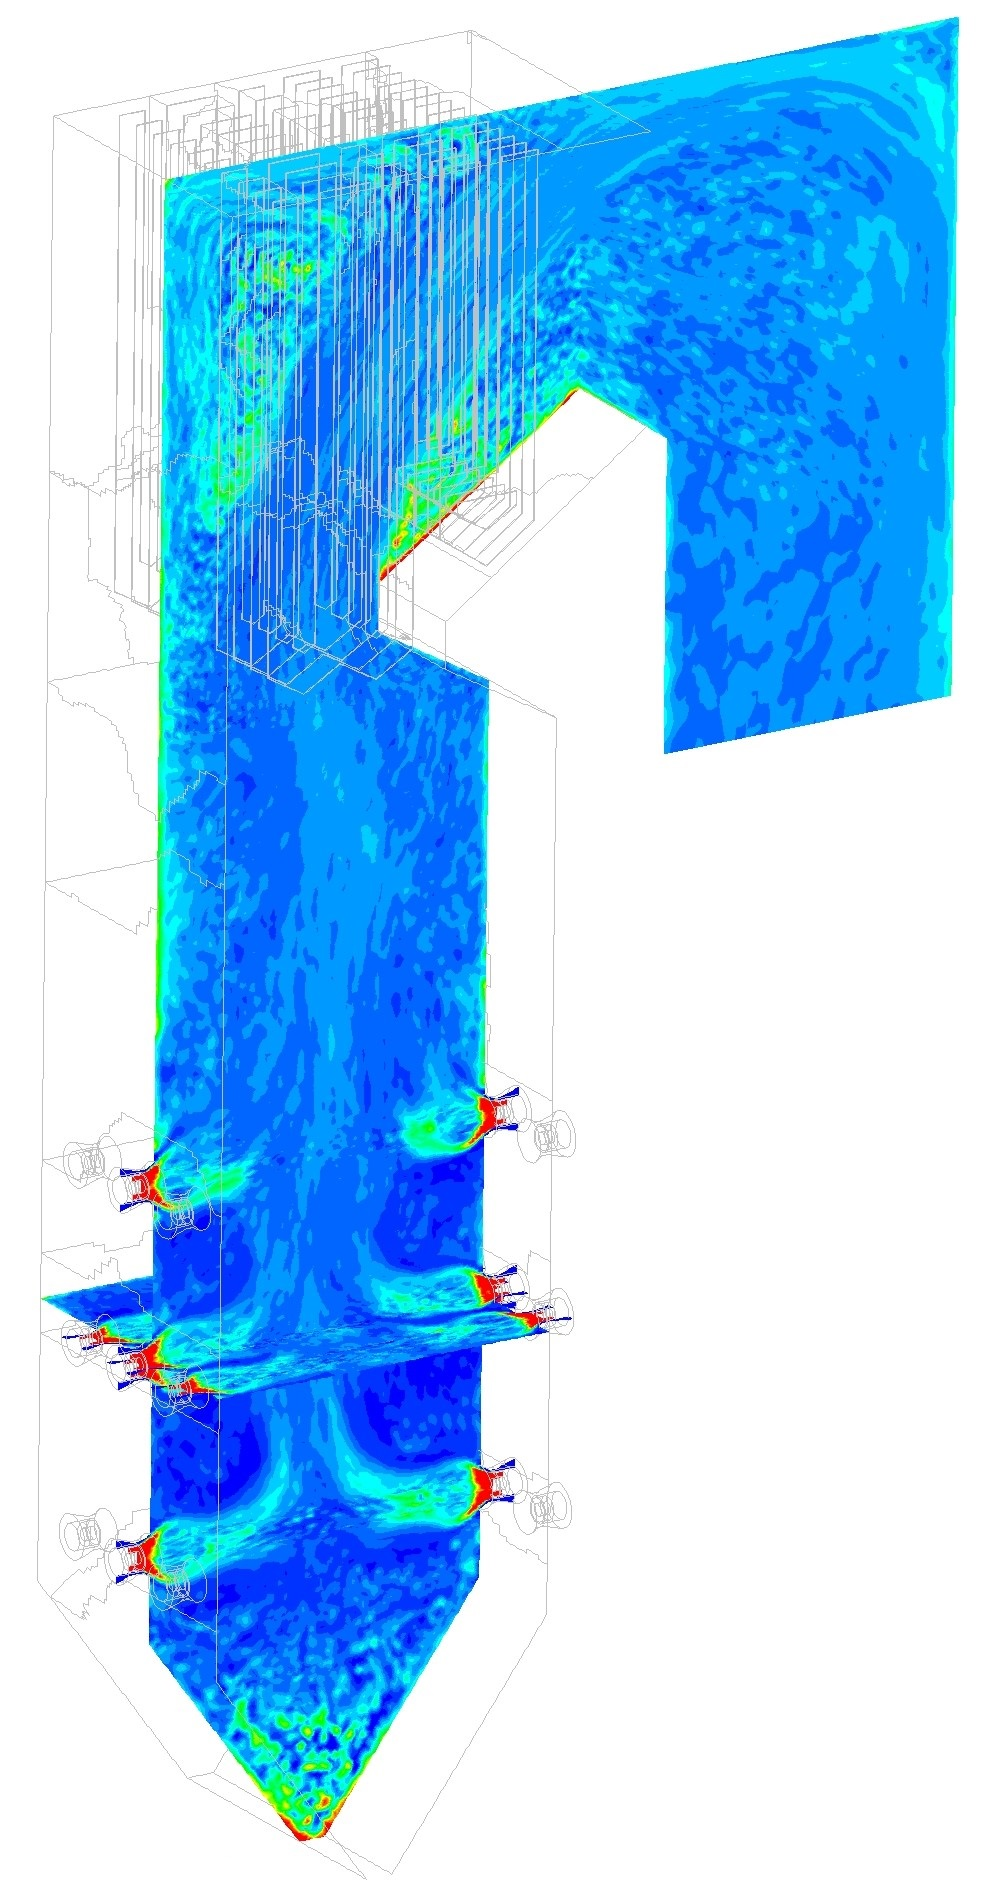
\includegraphics[scale = 0.085]{60_concentration}}\\
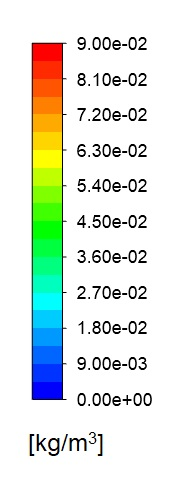
\includegraphics[scale = 0.3]{concentration}
\subfloat[100\% case]{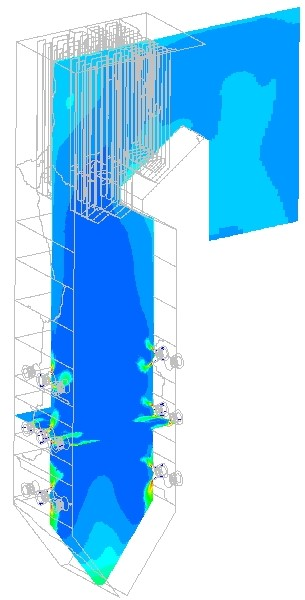
\includegraphics[scale = 0.27]{100_concentration_spm}}
\hspace{10mm} 
\subfloat[100\% case]{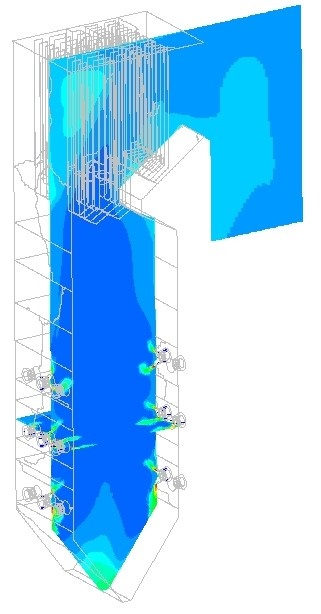
\includegraphics[scale = 0.27]{80_concentration_spm}}
\hspace{10mm}  
\subfloat[100\% case]{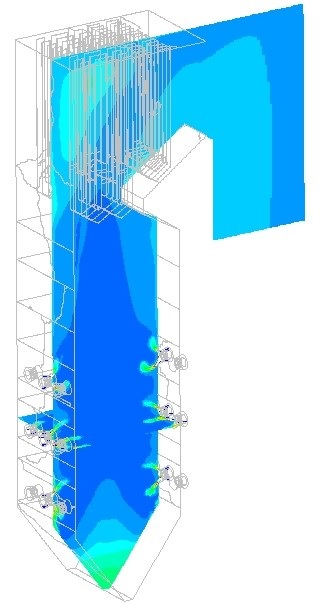
\includegraphics[scale = 0.27]{60_concentration_spm}}
\setlength{\belowcaptionskip}{0pt} 
\caption{Spatial particle concentration profiles for the numerical (a-c) and EE model (d-f) simulated load cases}
\label{fig_concentration}
\end{figure}

\section{Conclusion}
The validation of a full scale 620 MWe boiler was conducted using a non-thermal equilibrium Eulerian-Eulerian model for three load cases, namely 100\%, 81\% and 60\% steady-state loads. The valdiation cases include a comparison to numerical model using a Eulerian-Lagrangian aprroach and where applicable measured site data.\\
\\
The developed EE model demonstrated adequate performance in predicting the flow profiles, wall heat fluxes and fluid property distributions throughout the domain.\\
\\
The computational speedup, of 30\%, from using the EE model was shown to a beneficial attribute when considering the development of a data-driven surrogate model. The relative accuracy of the EE model ranged from 2 to 8\% for key parameters used in the study.

\section*{Acknowledgements}
The authors would like to thank the Eskom EPPEI program for funding this project and the Centre for High Performance Computing (CHPC, South Africa) for the computational resources provided for completing this work.

%
% BibTeX or Biber users please use (the style is already called in the class, ensure that the "woc.bst" style is in your local directory)
% \bibliography{name or your bibliography database}
%
% Non-BibTeX users please use
%
\newpage



\begin{thebibliography}{}
%
% and use \bibitem to create references.
%

\bibitem{bohnstein}
von Bohnstein, M., Richter, M., Graeser, P., Schiemann, M. and Str{\"{o}}hle, J. and Epple, B., Renewable and Sustainable Energy Reviews \textit{CFD (Computational fluid dynamics),Oxy-fuel combustion,Radiation modelling,Weighted-sum-of-gray-gases model (WSGGM)}, \textbf{137}, (2021)

\bibitem{laubscher_1}
Laubscher, R. and Rousseau, P., Applied Thermal Engineering - \textit{CFD study of pulverized coal-fired boiler evaporator and radiant superheaters at varying loads}, \textbf{160}, (2019)

\bibitem{laubscher_2}
Laubscher, R. and Rousseau, P., International Journal of Heat and Mass Transfer - \textit{Numerical investigation into the effect of burner swirl direction on furnace and superheater heat absorption for a 620 MWe opposing wall-fired pulverized coal boiler}, \textbf{137}, 506-522 (2019)

\bibitem{cai}
Cai, J., Handa, M., and Modest, M.F., Combustion and Flame - \textit{Eulerian-Eulerian multi-fluid methods for pulverized coal flames with nongray radiation}, \textbf{162}, 1550-1565 (2015)

\bibitem{wu}
Wu, Y., Liu, D., Ma, J., and Chen, X., Powder Technology - \textit{Effects of gas-solid drag model on Eulerian-Eulerian CFD simulation of coal combustion in a circulating fluidized bed}, \textbf{342}, 48-61 (2018)

\bibitem{epple}
Benim, A.C., Epple, B. and Krohmer, B., Progress in Computational Fluid Dynamics - \textit{Eulerian-Eulerian modelling of two-phase flow,Pulverised coal combustion}, \textbf{5}, 345-361 (2005)

\bibitem{knaus}
Knaus, H. , Schnell, U. and  Klaus R.G., Progress in Computational Fluid Dynamics - \textit{On the modelling of coal combustion in a 550MWe coal fired utility boiler} , \textbf{1}, 194–207 (2001)

\bibitem{shih}
Shih, T.H., Liou, W.W., Shabbir, A., Wang, Z. and Zhu, J., Computers and fluids - \textit{A new k-epsilon eddy viscosity model for high reynolds number turbulent flows}, \textbf{24}, (1995)


\bibitem{cengel}
Cengel, Y.A. and Boles, M.A., \textit{Thermodynamics: An engineering approach}, (McGraw Hill, Singapore, 2015)


\bibitem{gupta}
Ranade, Vivek V. and Gupta, Devkumar F., \textit{Computational Modeling of Pulverized Coal Fired Boilers}, (CRC Press - Taylor {\&} Francis Group, Boca Raton, 2015) 101-105


\bibitem{sankar}
Sankar, G., Santhosh Kumar, D. and Balasubramanian, K.R., Fuel -\textit{Computational modeling of pulverized coal fired boilers – A review on the current position}, \textbf{236}, 643-665 (2019)

\bibitem{baum}
Baum, M.M. and Street, P.J.,Combustion Science and Technology -\textit{Predicting the Combustion Behaviour of Coal Particles Predicting the Combustion Behaviour of Coal Particles}, \textbf{3}, 231-243 (1971) 


\bibitem{spalding}
Spalding, D.B., Symposium (International) on Combustion - \textit{Mixing and Chemical Reaction in Steady Confined Turbulent Flames}, \textbf{13}, (1970)


\bibitem{ansys}
\textit{ANSYS Fluent Theory Guide}, (Ansys Inc., 2021)

\bibitem{smith}
Smith T., Shen Z., and Firedman J., Journal of Heat Tranfer - \textit{Evaluation of Coefficients for the Weighted Sum of Gray Gases Model}, \textbf{104}, 602-608 (1982)

\bibitem{laubscher_3}
Laubscher, R. and Rousseau, P., Energy - \textit{Numerical investigation on the impact of variable particle radiation properties on the heat transfer in high ash pulverized coal boiler through co-simulation}, \textbf{195}, (2020)




% etc
\end{thebibliography}

\end{document}

% end of file template.tex

<div id='footer'><table width='100%'><tr><td class='right'><a href='http://fusioninventory.org/'><span class='copyright'>FusionInventory 9.1+1.0 | copyleft <img src='/glpi/plugins/fusioninventory/pics/copyleft.png'/>  2010-2016 by FusionInventory Team</span></a></td></tr></table></div>